\documentclass{article}
\usepackage{polski}
\usepackage[utf8]{inputenc}
\usepackage[a4paper, total={6in, 9in}]{geometry}
\usepackage{changepage}
\usepackage{graphicx}
\usepackage{multicol}
\usepackage{blindtext}

\setlength{\columnsep}{1cm}
\graphicspath{ {../data/plots/} }

\title{Algorytmy Metaheurystyczne\\Tabu Search}
\author{Piotr Puszczyński 254620\\Michał Krosny 256791}

\begin{document}

\maketitle
\newpage

\section{Działanie algorytmu}

Algorytm tabu search został zaimplementowany w obiektowym jezyku c++ z
założeniem możliwości rozszerzenia o interfejsy dla innych problemów niż
TSP. Pozwala na to rozbudowany schemat dziedziczenia z klas Solutnion czy Problem
jak i mocno sparametryzowany schemat rozwiązywania problemu. Dodatkowo program jest
zoptymalizowany pod kątem obliczeń wielowątkowych\\
Kryterium aspiracji jest po porstu znalezienie lepszego rozwiązania niż akutalnie najlepsze.
Kryterium stagnacji to maksymalna liczba iteracji, iteracji bez poprawy lub przeszukanie
całego otoczenia od najlepszego uzyskanego wyniku.

Program przyjmuje na wejście nazwę pliku (po fladze -input) instancji TSP w postaci macierzy i pozwala
na sparametryzowanie sposobu rozwiązywania problemu przy pomocy następujących flag:\\
\begin{itemize}
    \item -input plik macierzy instancji
    \item -path\_input plik ze ścieżką początkową
    \item -max\_iter maksymalna globalna liczba iteracji
    \item -max\_depth maksymalna liczba iteracji bez poprawy do nawrotu
    \item -max\_imp\_iter maksymalna liczba iteracji bez poprawy
    \item -max\_tabu maksymalna wielkość tabu
    \item -threads liczba wątków na których ma działać program
    \item -mode sposób znajodwania sąsiedztwa
    \item -clear\_tabu flaga oznaczająca czy algorytm ma czyścić tabu po osiągnięciu max\_depth
    \item -print\_debug flaga zmieniająca tryb na tryb debugowania (wypisuje numer iteracji w której algorytm znalazł lepszą ścieżkę)
\end{itemize}

\noindent Za parametry standardowe dla instancji wielkości $n$ przyjęto:\\
\begin{itemize}
  \item Wielkość tablicy tabu $= \lceil \sqrt{n} \rceil $
  \item Głębokość poszukiwań $= \lceil \sqrt{n} \rceil $
  \item Maksymalną liczbę iteracji bez poprawy $= 2 * n^2 $
  \item Maksymalną globalną liczbę iteracji $= 50000$
\end{itemize}

\section{Przeprowadzone badania}
Na algoryrmie przeprowadzono następujące badania:
\begin{enumerate}
  \item Wpłw wielkości instancji dla postawowych parametrów na czas oraz PRD
  \item Wpływ doboru wielkości tablicy tabu do PRD oraz czasu
  \item Wpływ doboru głębokości poszukiwań do PRD
  \item Wpływ doboru ilości iteracji bez poprawy przed terminacją do PRD
\end{enumerate}

Wszystkie badania zostały przeprowadzone w zależności od użytej instancji z bliblioteki
TSPLib oraz dodatkowo dla instancji losowych z uśrednioną wartością dla danej wielkości problemu.
Każdy z testów został przetestowany dla 3 sposobów określania sąsiedztwa: Invert Swap oraz Insert.
Badania gównie skupijają się na metodzie Invert.

\section{Wpływ wielkości instancji dla postawowych parametrów na czas oraz PRD}

Na wykresach przedstawiono zależność czasu od wielkości instancji oraz dla dobranego problemu
z bliblioteki TSPLib
\begin{adjustwidth}{-5cm}{-5cm}
  \begin{center}
    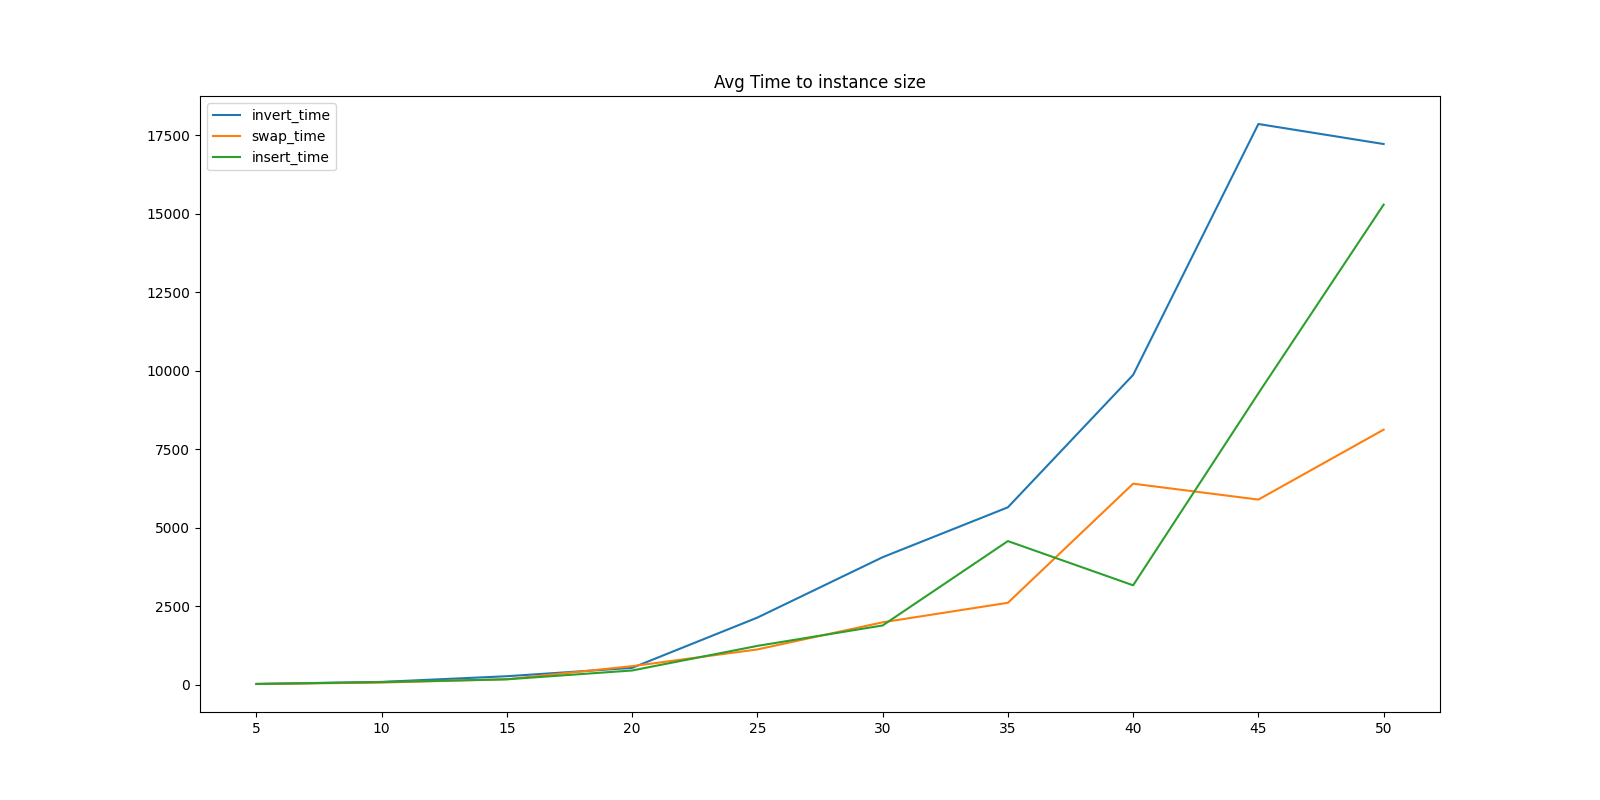
\includegraphics[scale=0.45]{rand_time.png}
  \end{center}
\end{adjustwidth}

\begin{adjustwidth}{-5cm}{-5cm}
  \begin{center}
    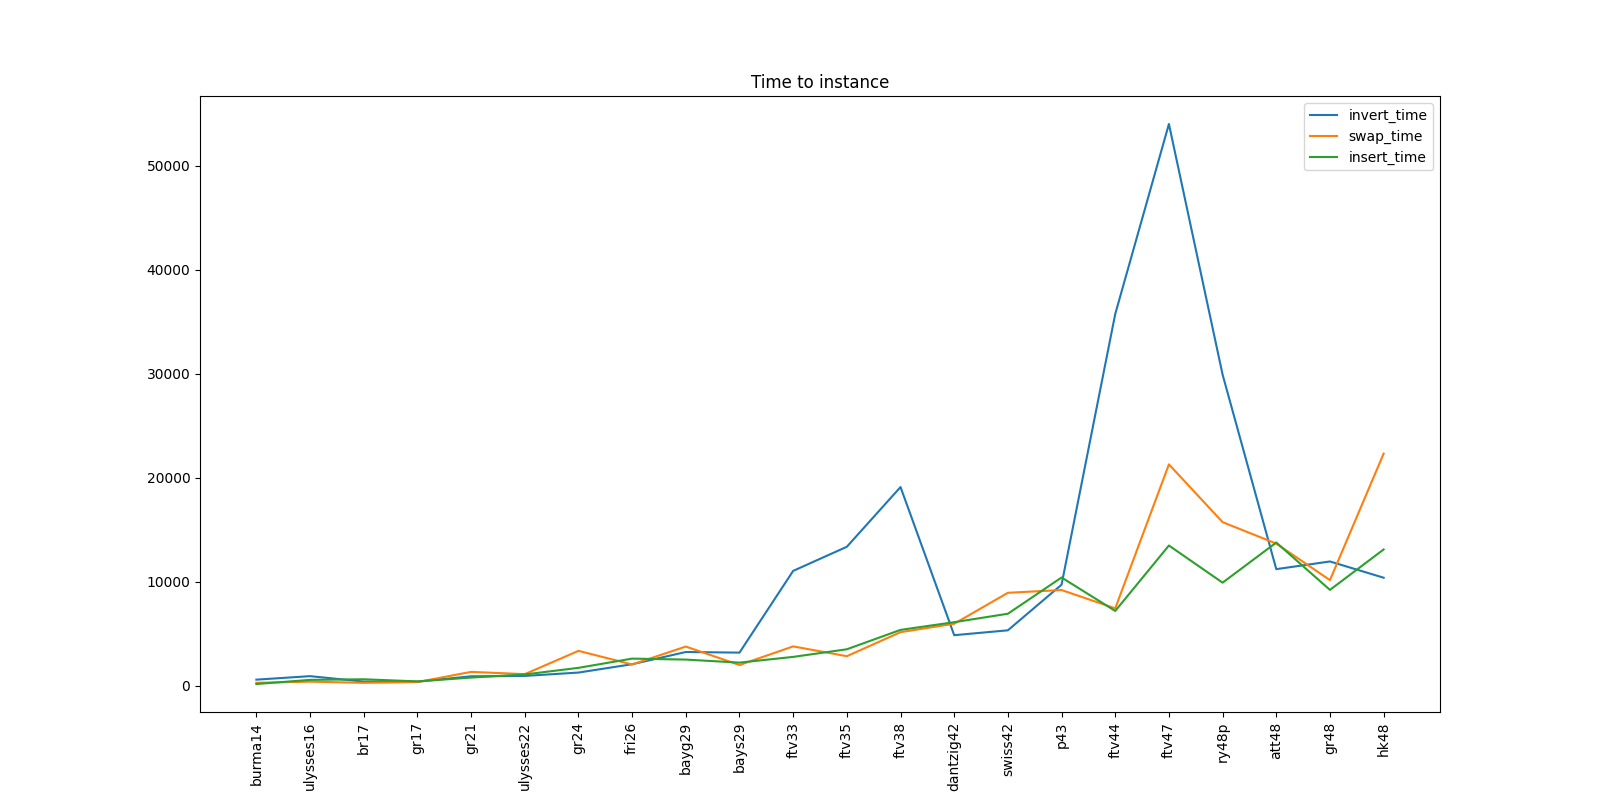
\includegraphics[scale=0.45]{time.png}
  \end{center}
\end{adjustwidth}

Łatwo zauważyć że dla większych problemów algortytmy przeważnie potrzebują
więcej czasu. Dodatkowo widać iż prostsze metody doboru sąsiedztwa czyli
Swap oraz Insert potrzebowały mniej czasu oraz analogicznie trudniejsza czyli invert
najwięcej czasu.\\
Dodatkowo widać, iż dla niektórych trudniejszych instancji czas wykonywania znacząco
się zwiększał.

\newpage

Wykresy przedstawiają wartości prd dla powyższych testów
\begin{adjustwidth}{-5cm}{-5cm}
  \begin{center}
    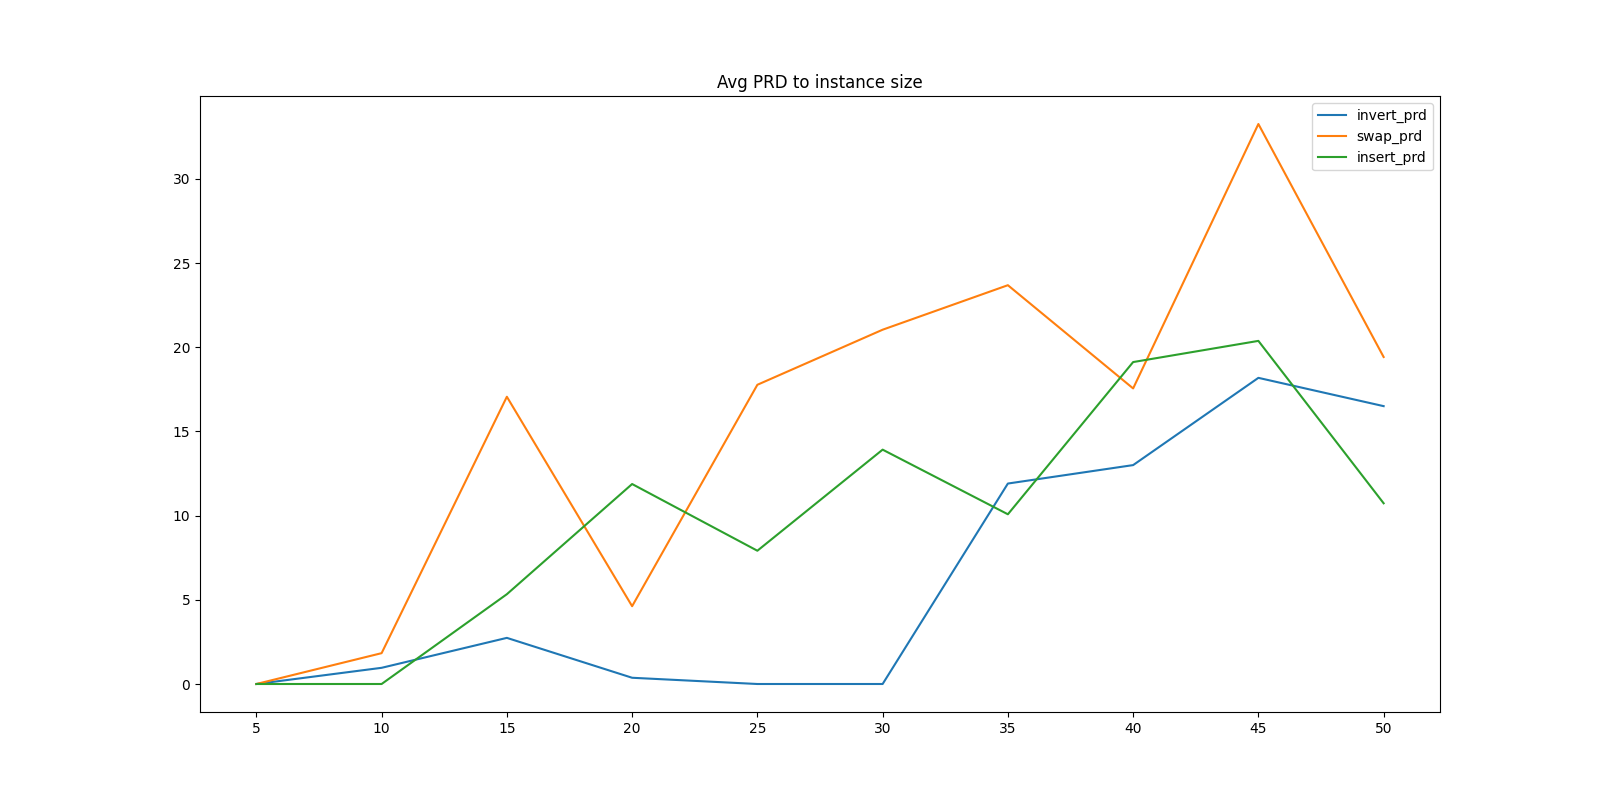
\includegraphics[scale=0.45]{rand_prd.png}
  \end{center}
\end{adjustwidth}

\begin{adjustwidth}{-5cm}{-5cm}
  \begin{center}
    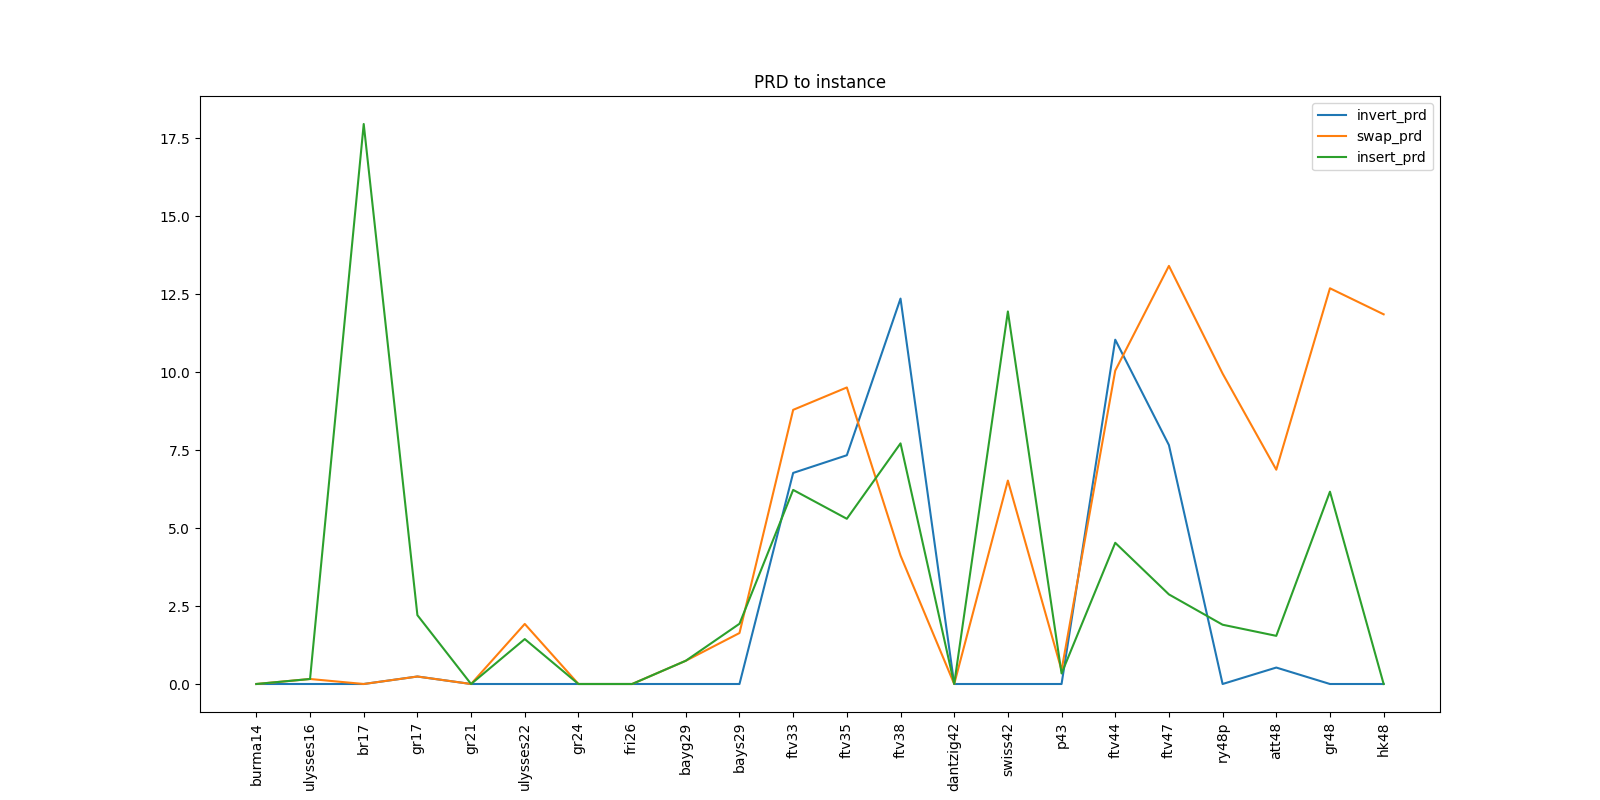
\includegraphics[scale=0.45]{prd.png}
  \end{center}
\end{adjustwidth}

Przeważnie metoda invert dawała najlepsze wyniki czesto najlepsze znane.
W przypadku instancji TSPLib w pojedyńczych przypadkach sprawdzała się ona gorzej
od pozostałych. Warto zauważyć że są to głównie instancje ftv co oznaczało by, że
jest to specyficzny problem i należało by przeprowadzić dalsze badania specyfiki tego
problemu.

\newpage
\section{Wpłw wielkości tablicy tabu na PRD oraz czas}
Na wykresach przedstawiono zależność czasu od wielkości losowych instancji dla różnych wielkośći listy tabu.

\begin{multicols}{2}
  \begin{center}
    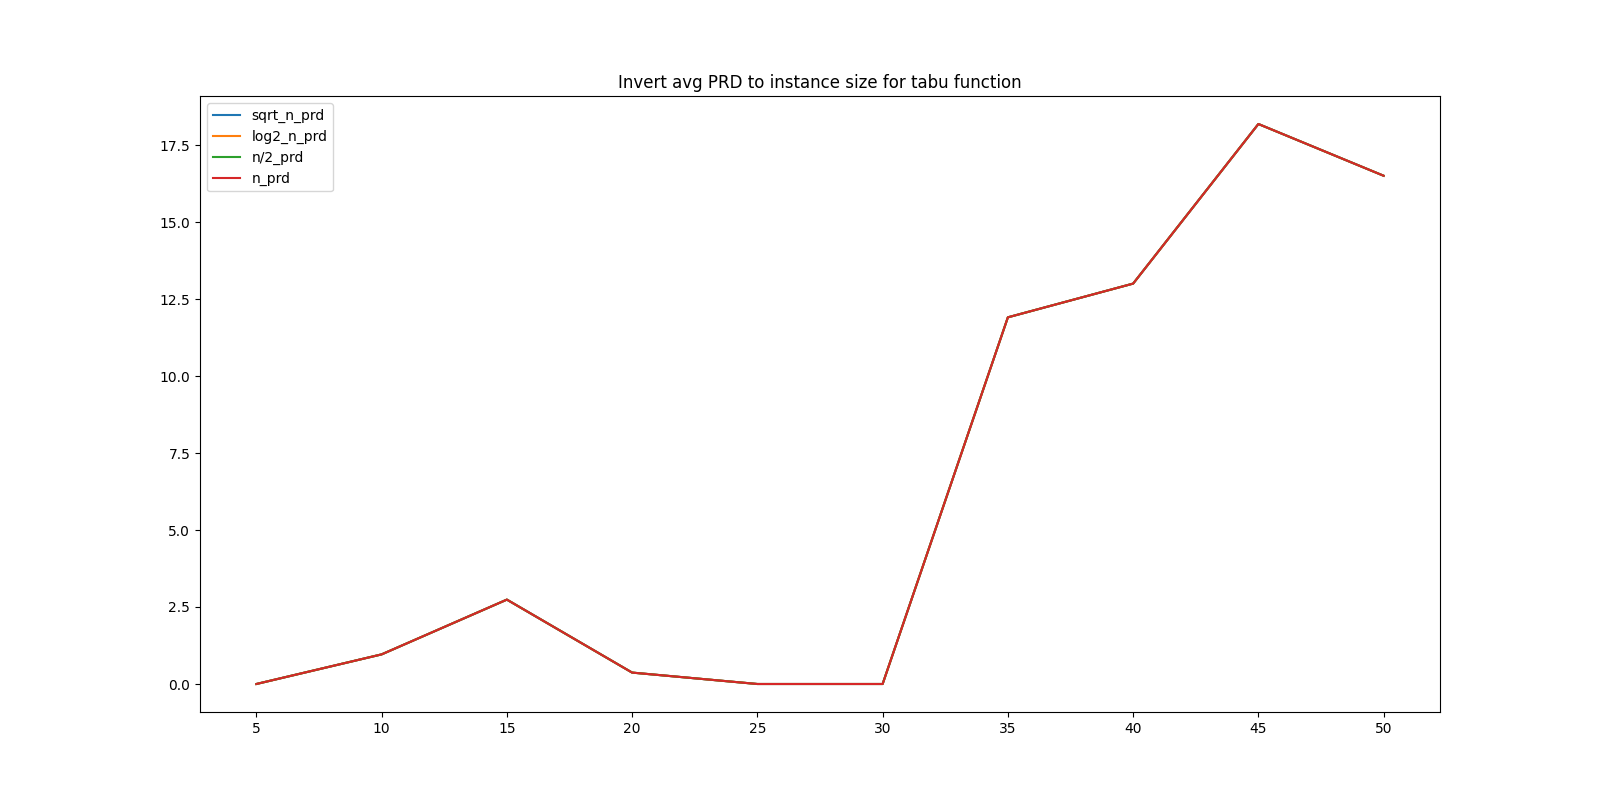
\includegraphics[scale=0.2]{rand_tabu_inv_prd.png}
    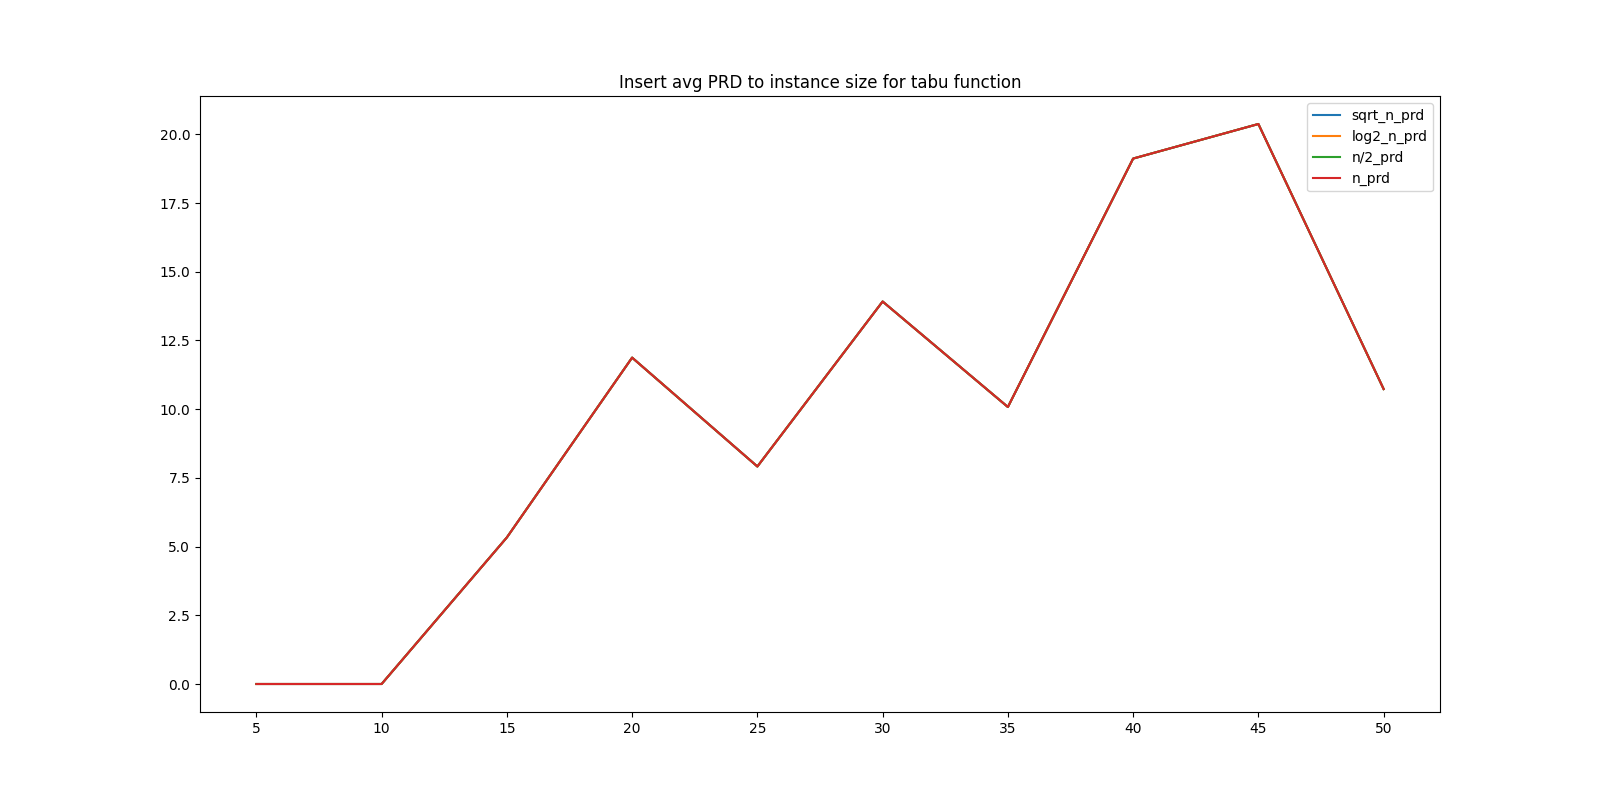
\includegraphics[scale=0.2]{rand_tabu_ins_prd.png}
    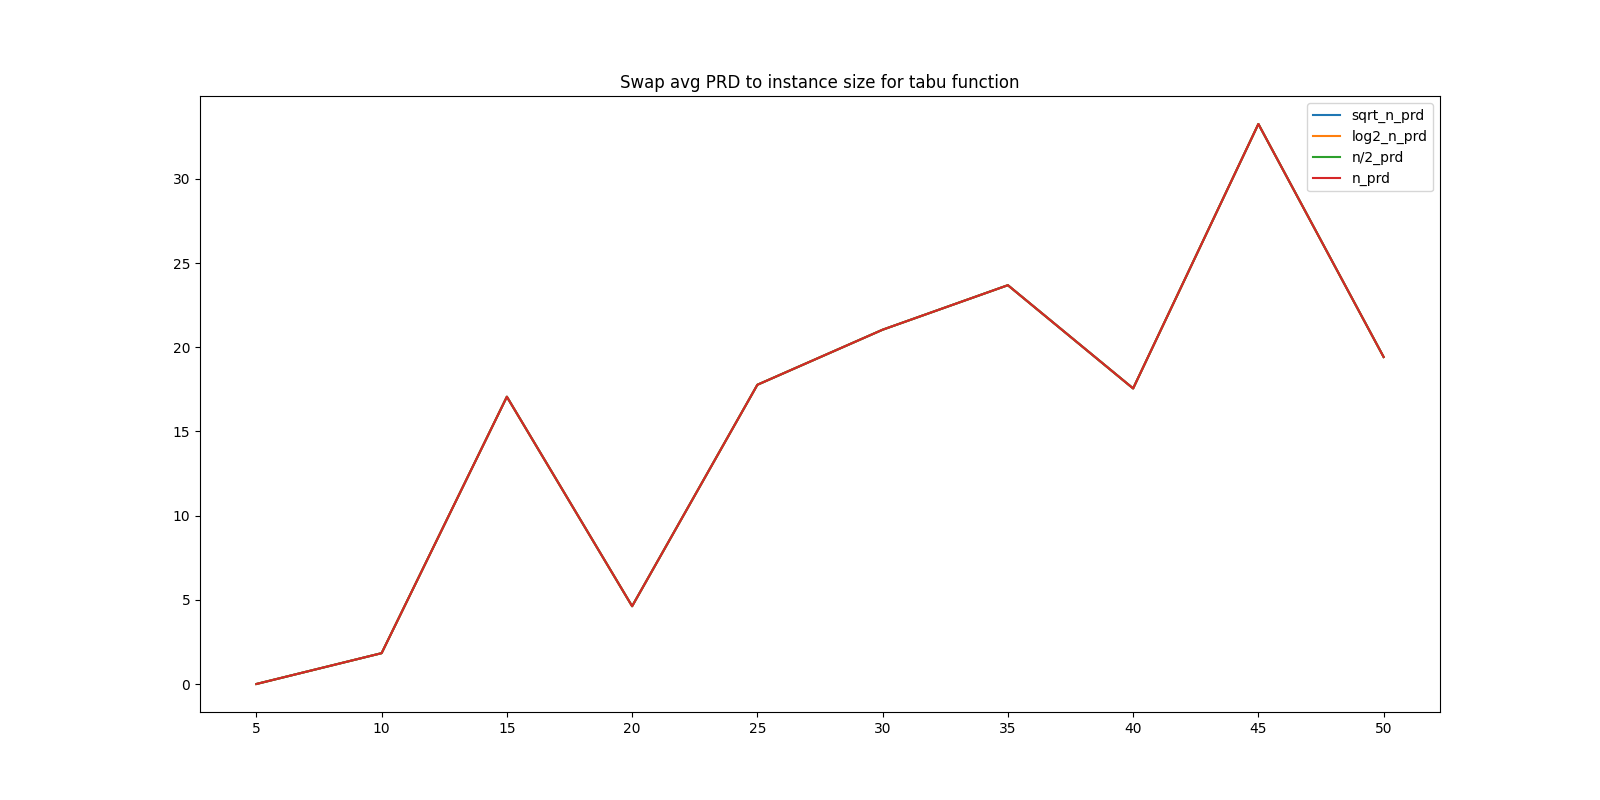
\includegraphics[scale=0.2]{rand_tabu_swp_prd.png}
    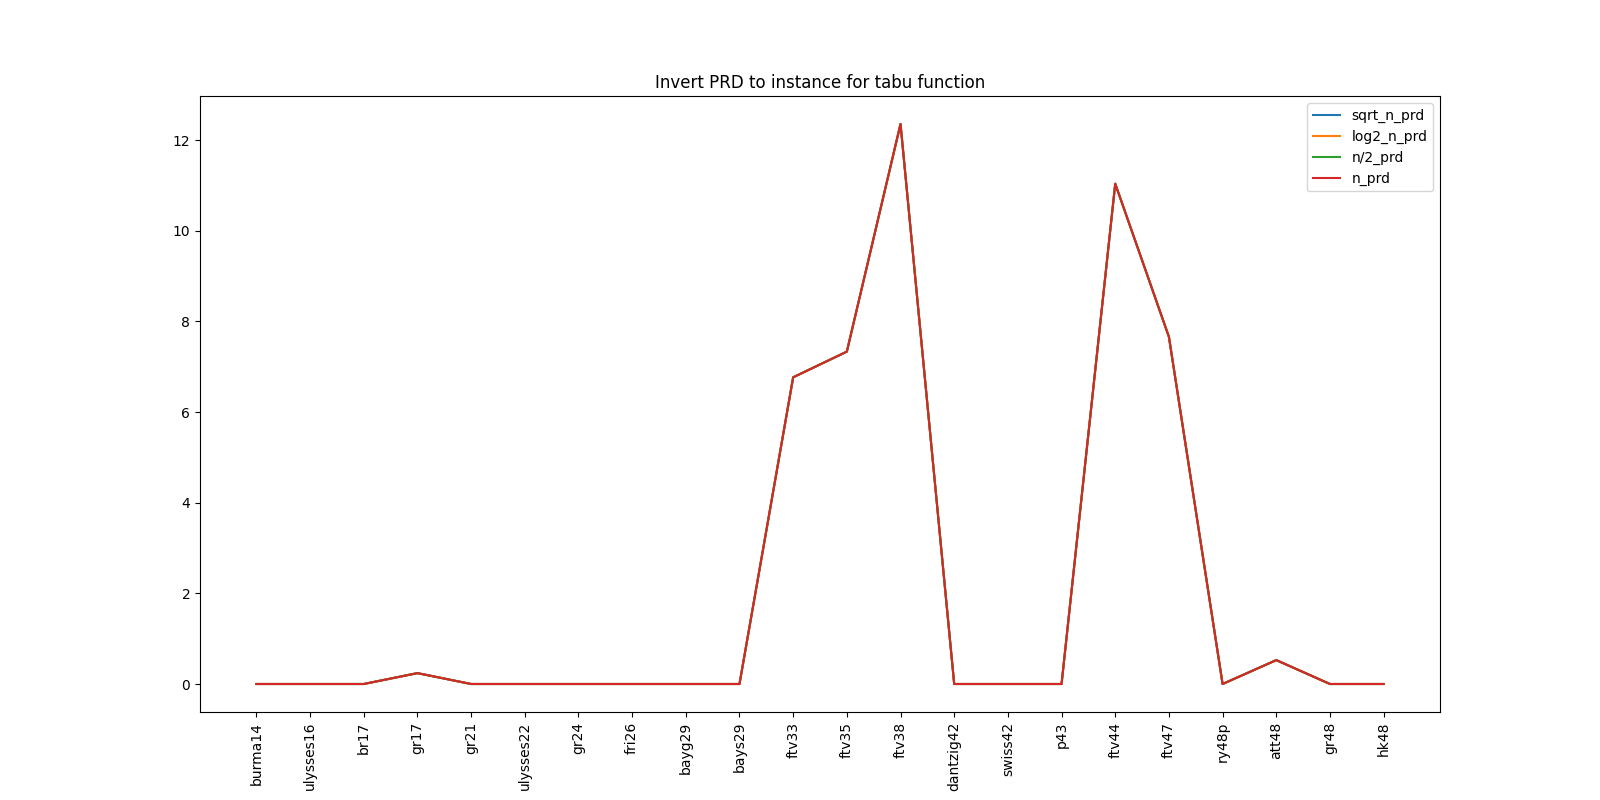
\includegraphics[scale=0.2]{tabu_inv_prd.png}
    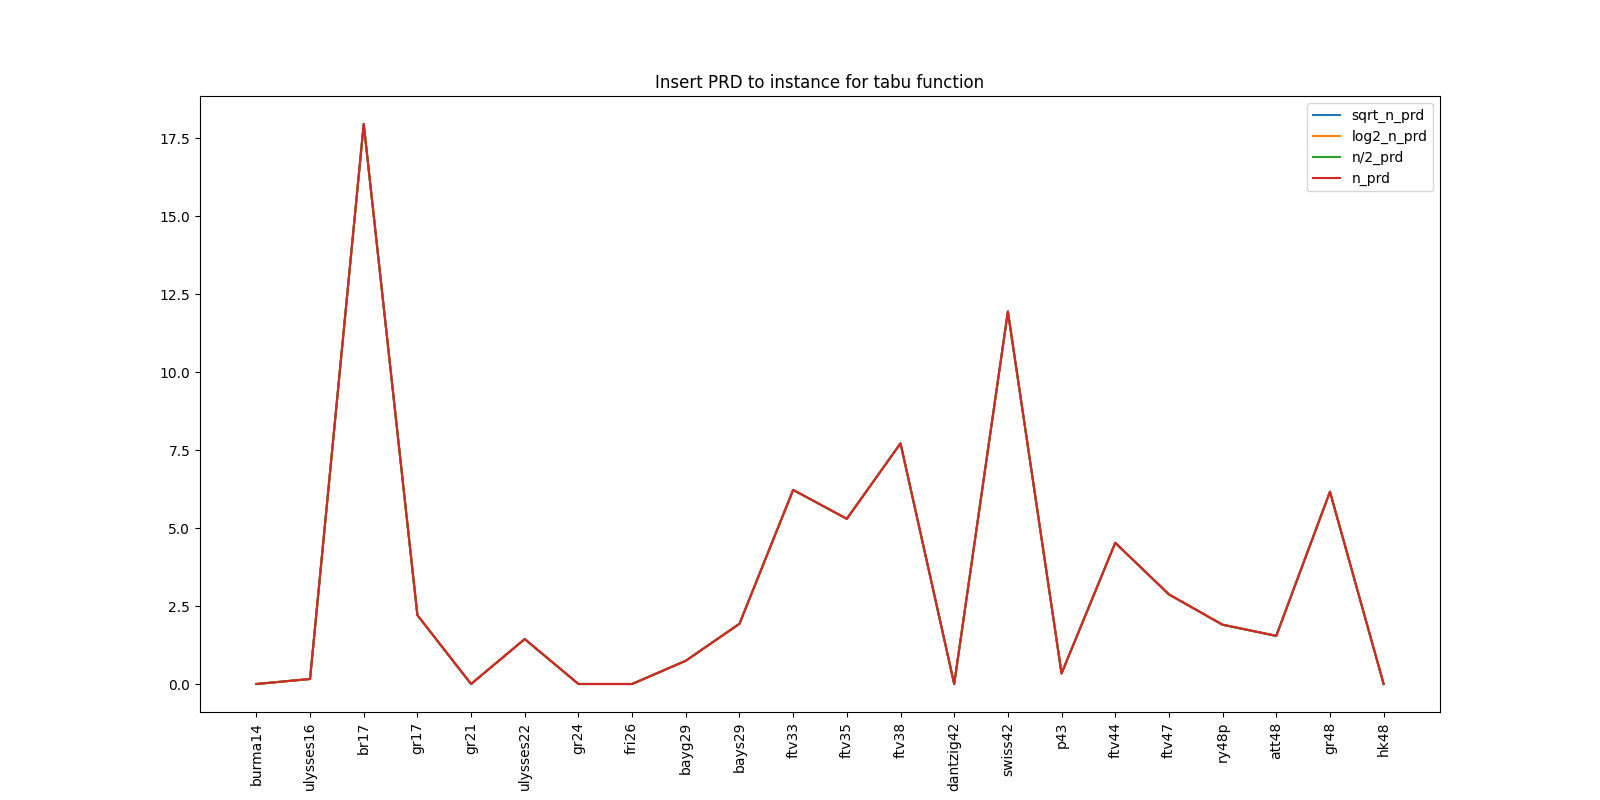
\includegraphics[scale=0.2]{tabu_ins_prd.png}
    \\~\\
    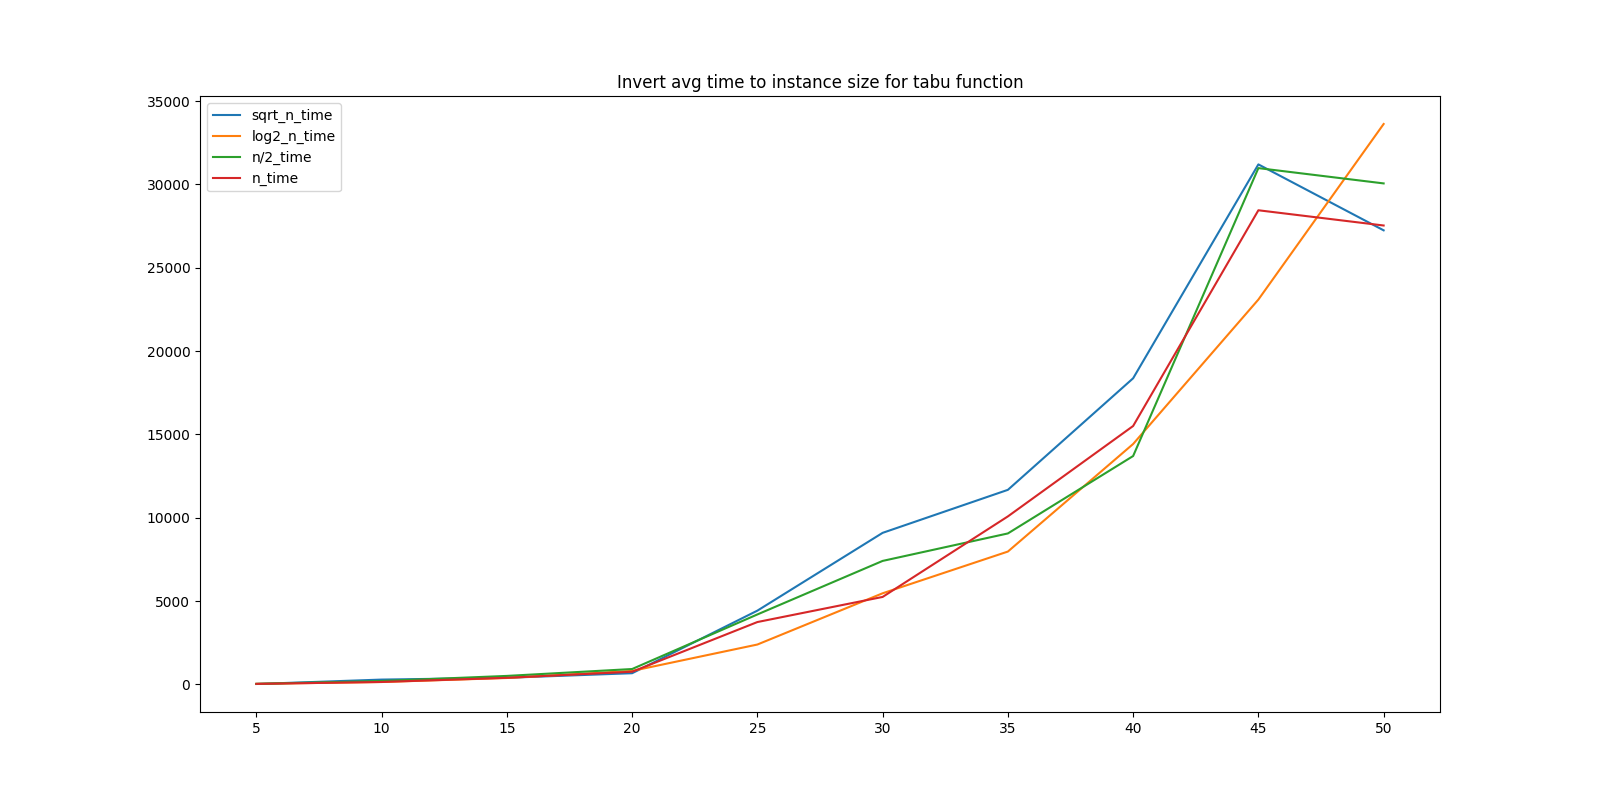
\includegraphics[scale=0.2]{rand_tabu_inv_time.png}
    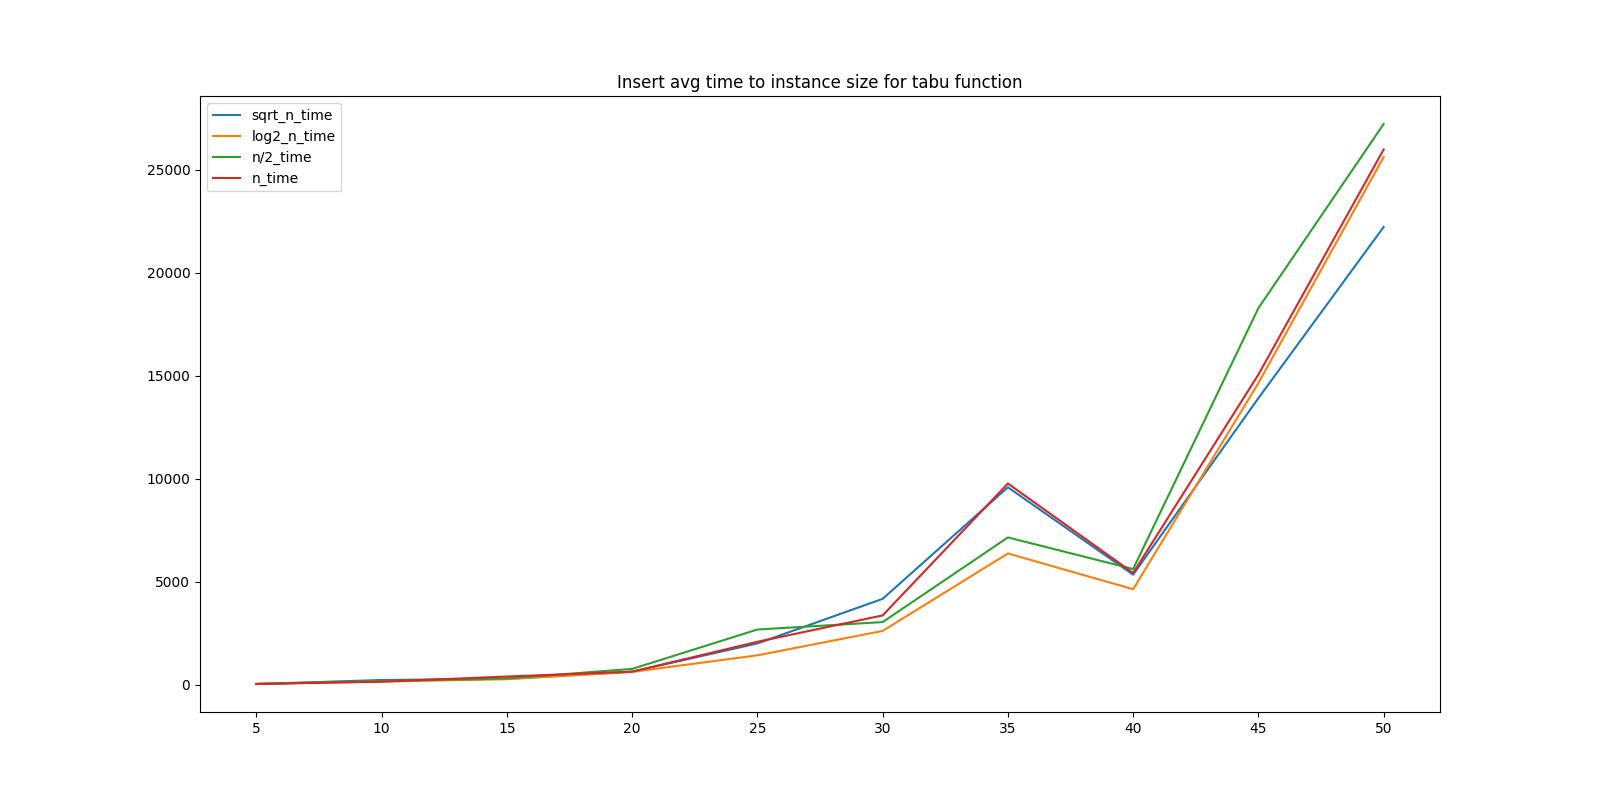
\includegraphics[scale=0.2]{rand_tabu_ins_time.png}
    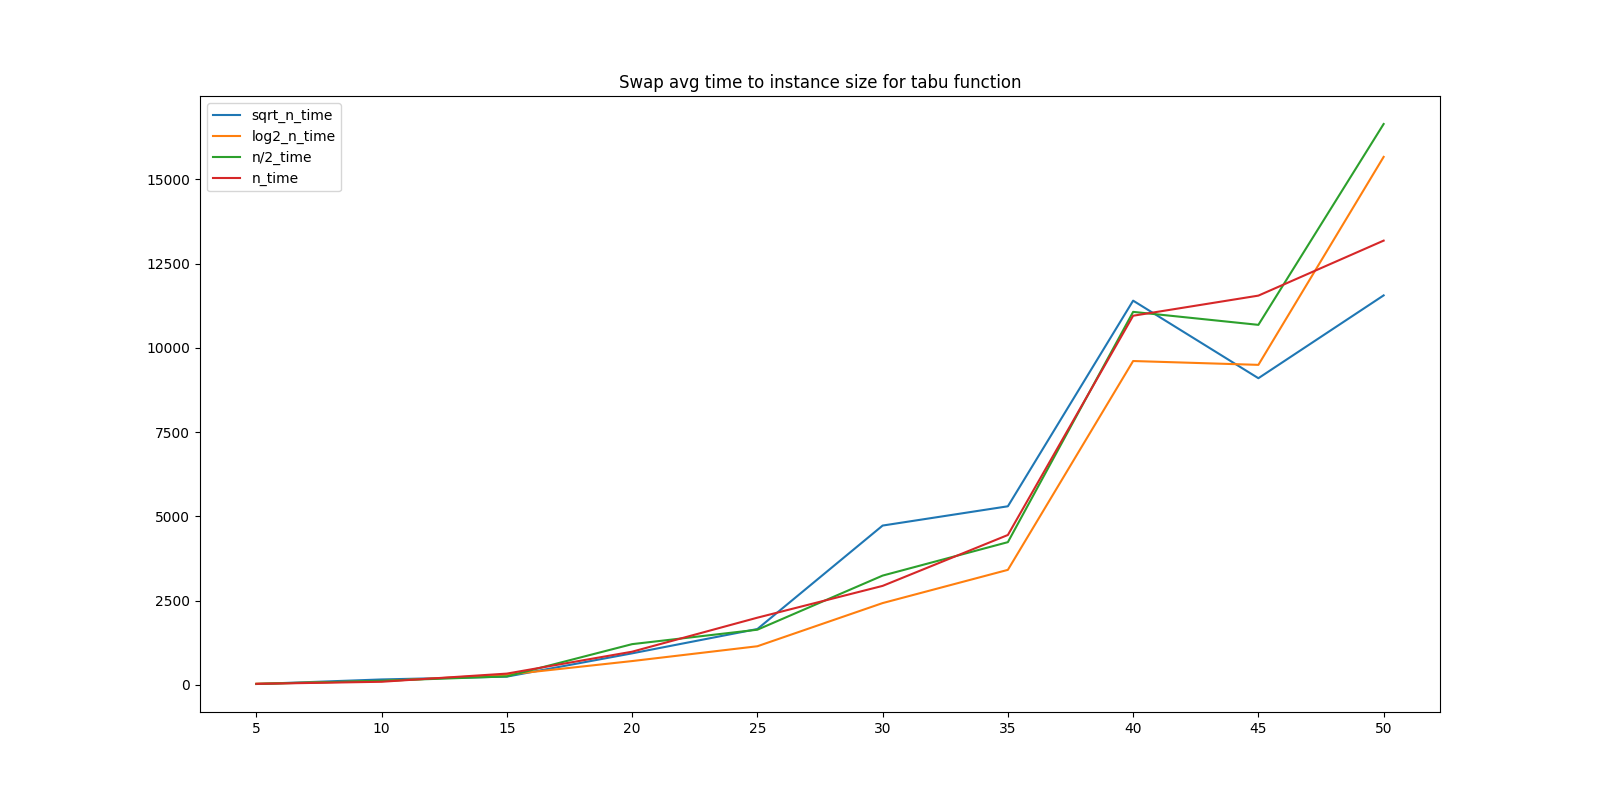
\includegraphics[scale=0.2]{rand_tabu_swp_time.png}
    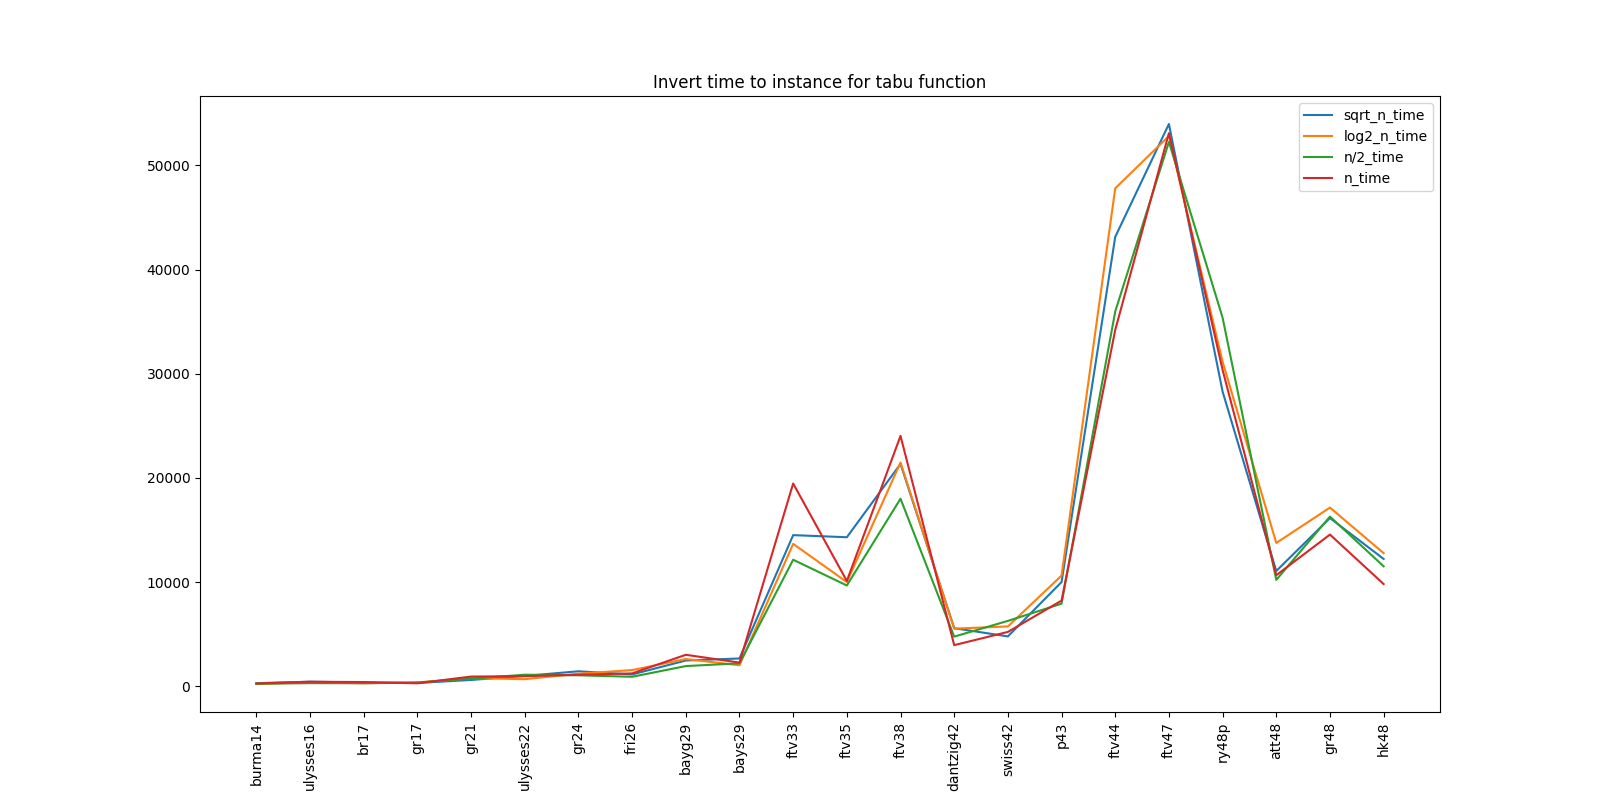
\includegraphics[scale=0.2]{tabu_inv_time.png}
    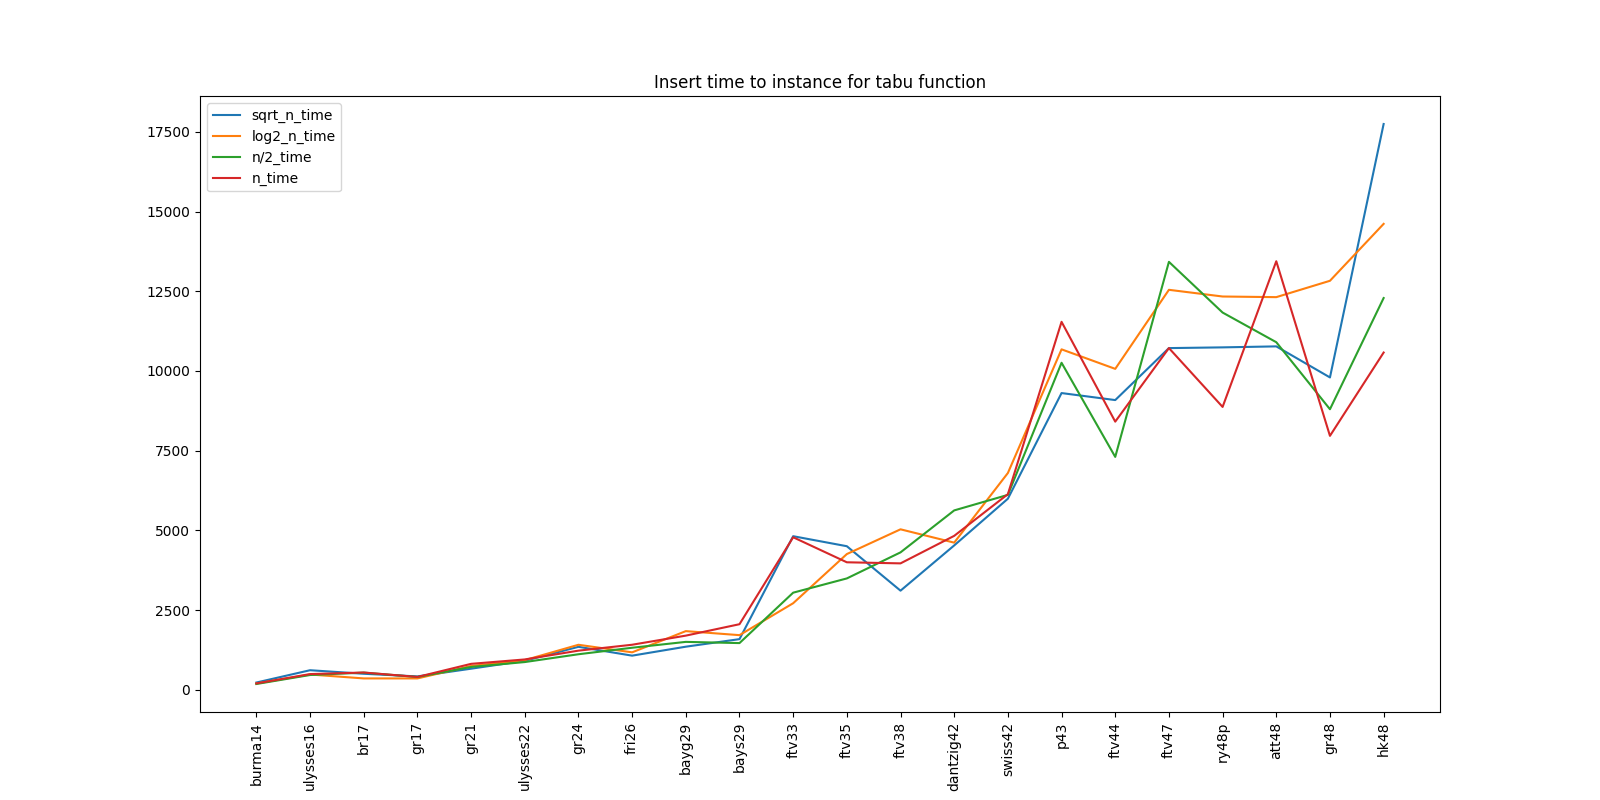
\includegraphics[scale=0.2]{tabu_ins_time.png}

  \end{center}
\end{multicols}

\begin{multicols}{2}
    \begin{center}
      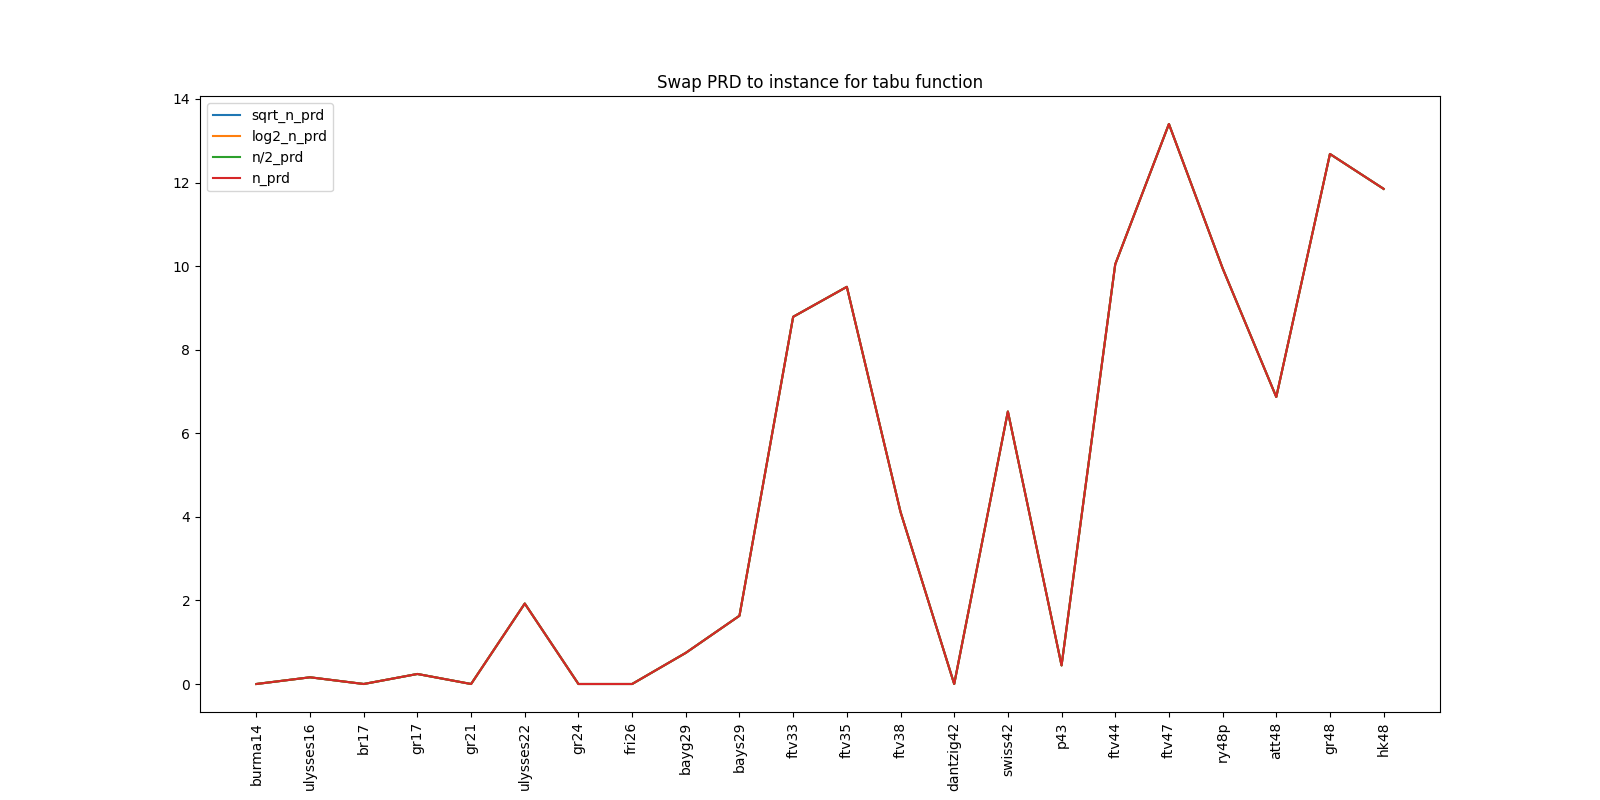
\includegraphics[scale=0.2]{tabu_swp_prd.png}
      \\~\\
      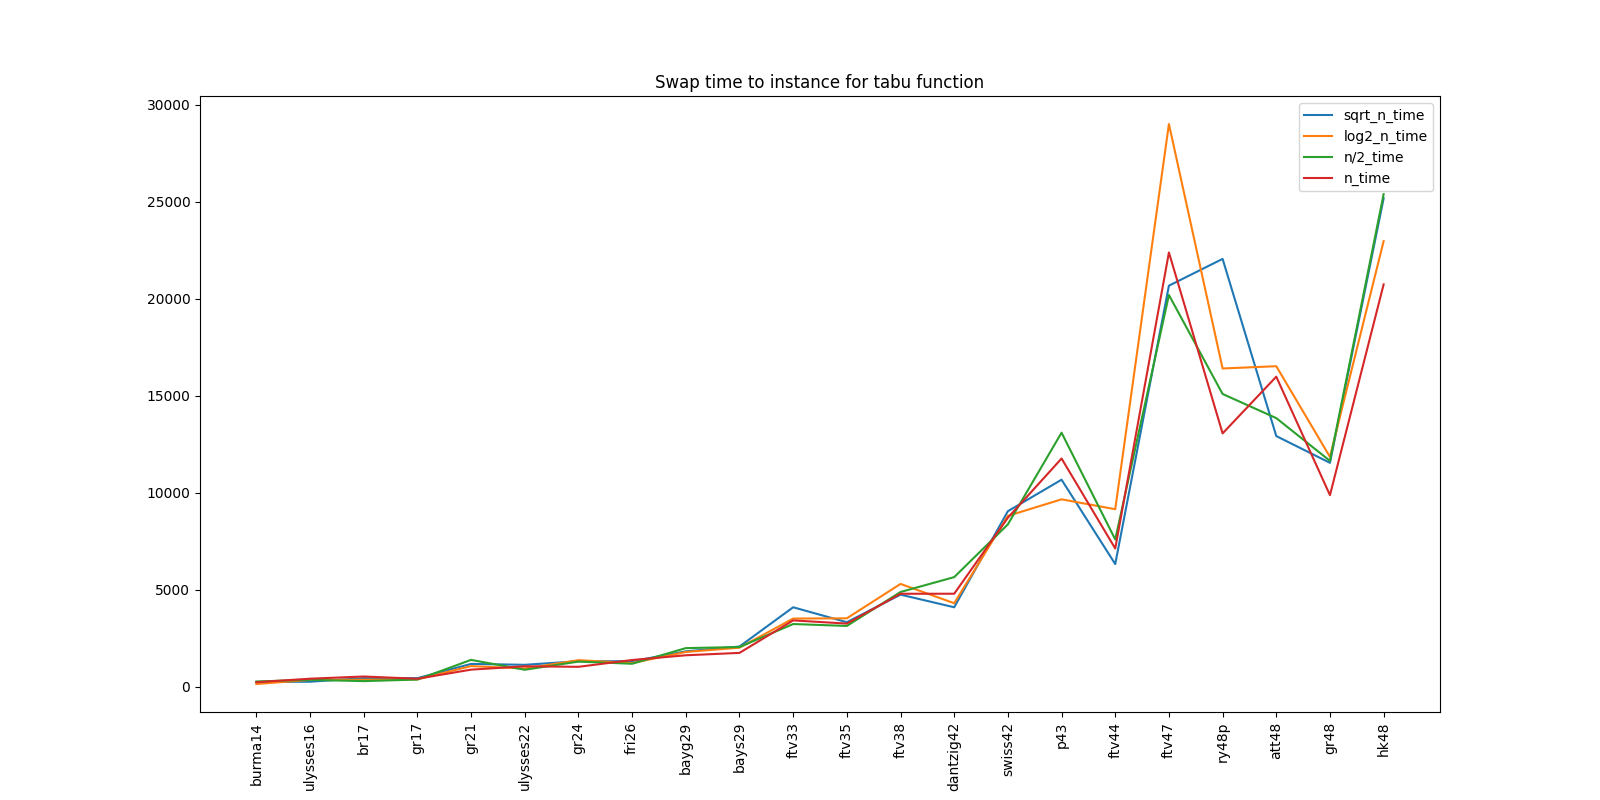
\includegraphics[scale=0.2]{tabu_swp_time.png}
    \end{center}
  \end{multicols}

  Przy wysatrczającej liczbie iteracji dla badanych funkcji wielkości tablicy wyniki są takie same, 
  jednak średni czas wykonywania znacząco się różni, najlepsze okazały się funkcje log i sqrt. Zasada ta działała
  głównie dla instancji losowych. W przypadku konkretnych instancji TSPLib należało by przprowadzić dalsze
  badania w celu znalezienia optymalnych funkcji wielkości tablicy tabu (prawdopodobnie zależnych od typu instancji)
%%


\section{Wpłw maksymalnej liczby iteracji bez poprawy do nawrotu na PRD}

Na wykresach przedstawiono zależność czasu od wielkości instancji dla różnych funkcji maksymalnych liczb iteracji bez poprawy do nawrotu.

\begin{multicols}{2}
    \begin{center}
      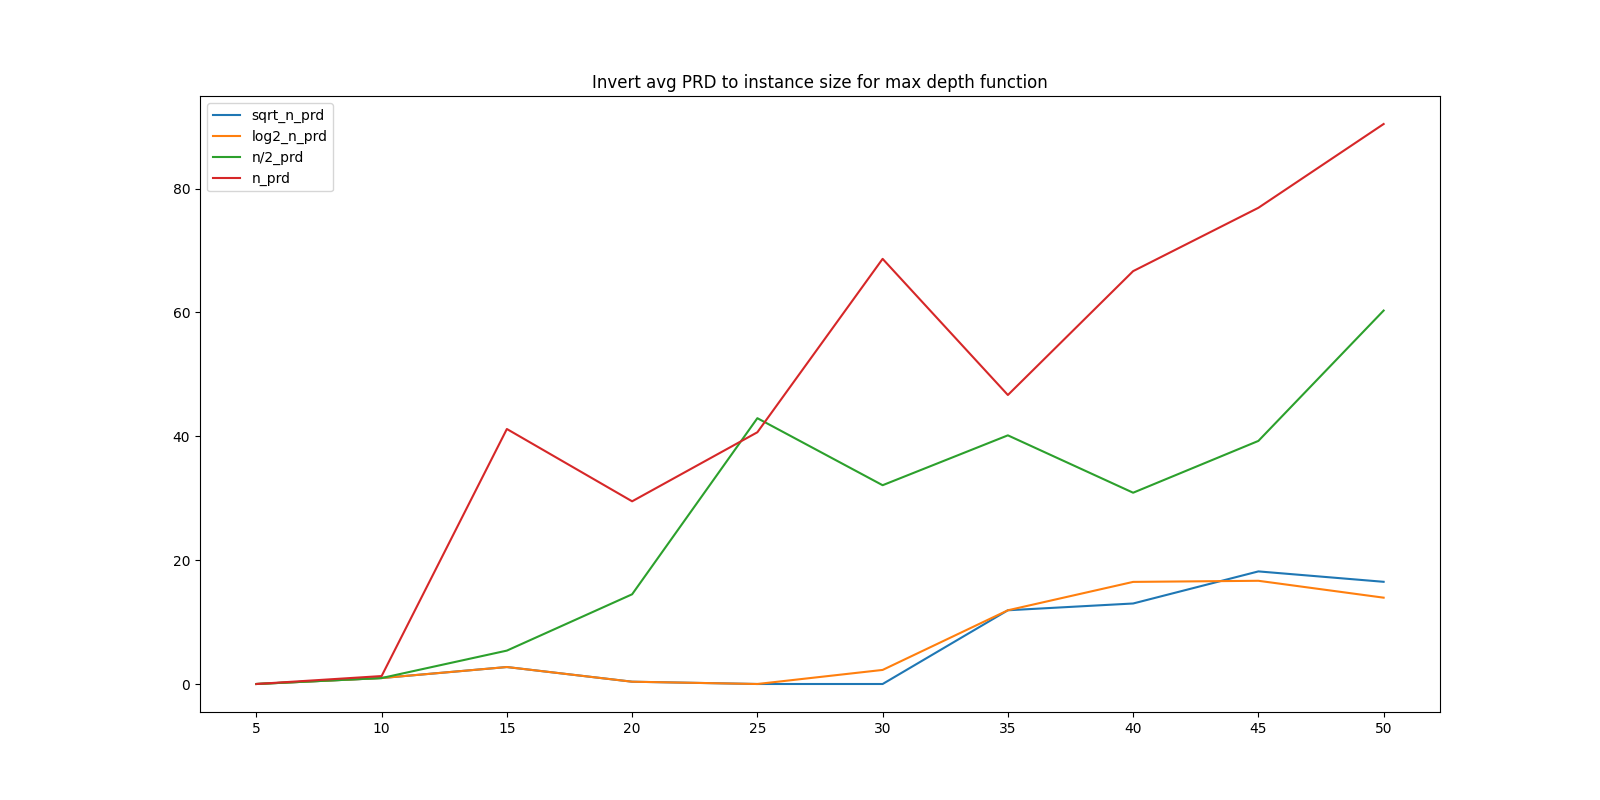
\includegraphics[scale=0.2]{rand_depth_inv_prd.png}
      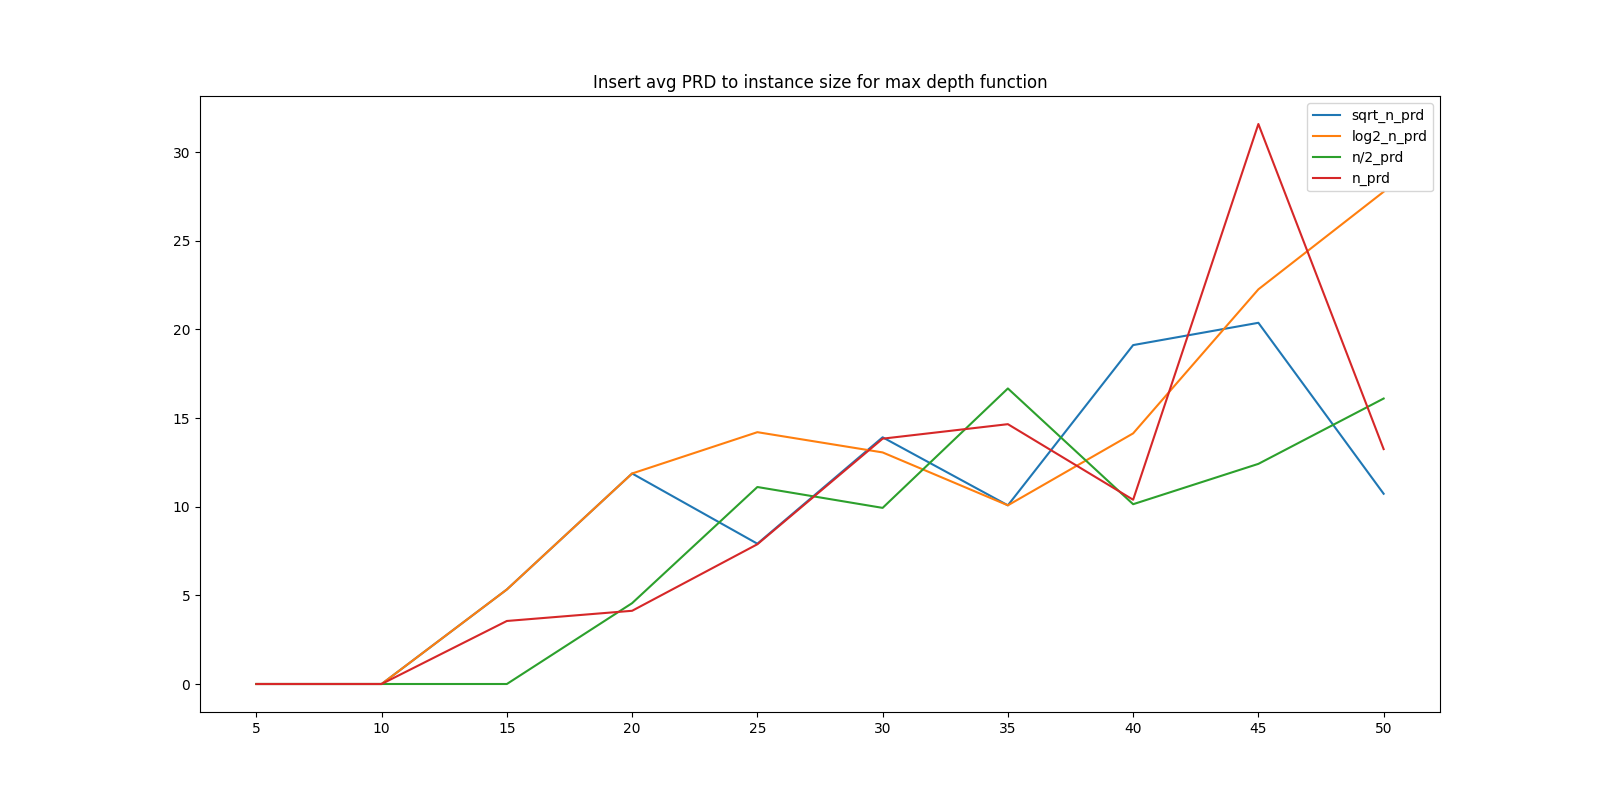
\includegraphics[scale=0.2]{rand_depth_ins_prd.png}
      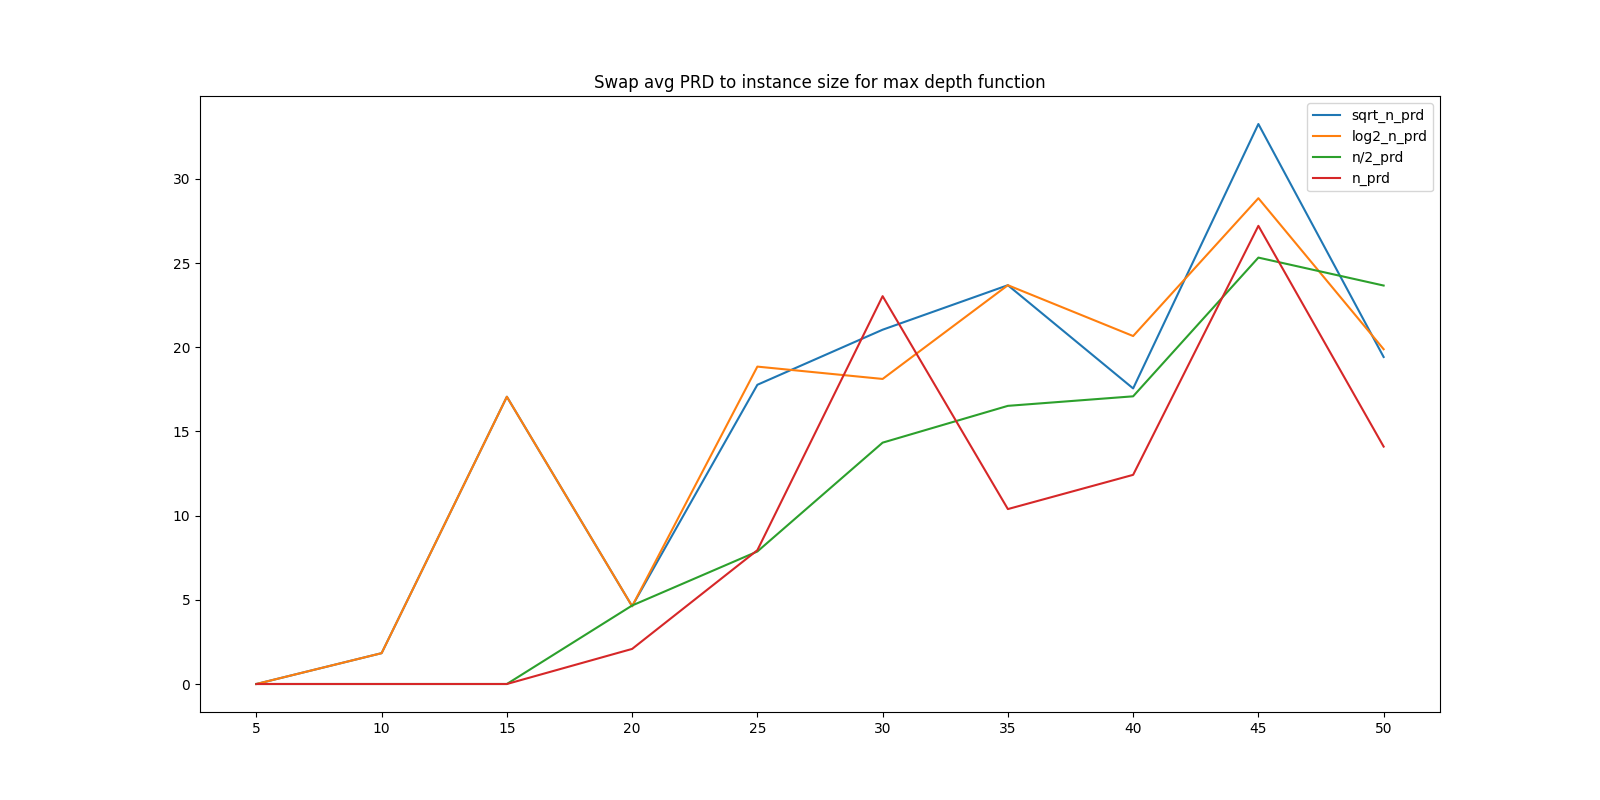
\includegraphics[scale=0.2]{rand_depth_swp_prd.png}
      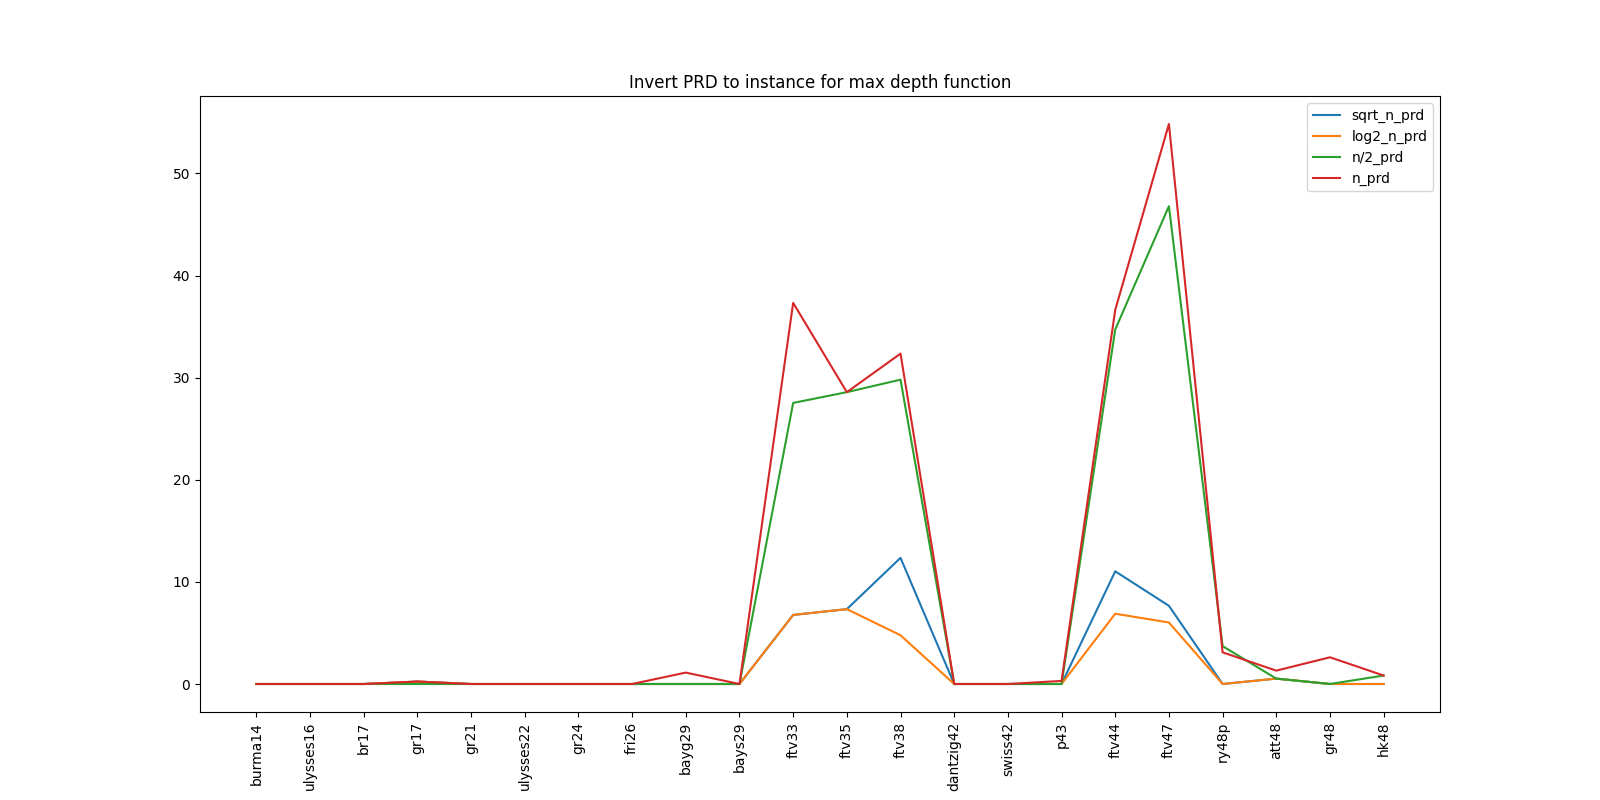
\includegraphics[scale=0.2]{depth_inv_prd.png}
      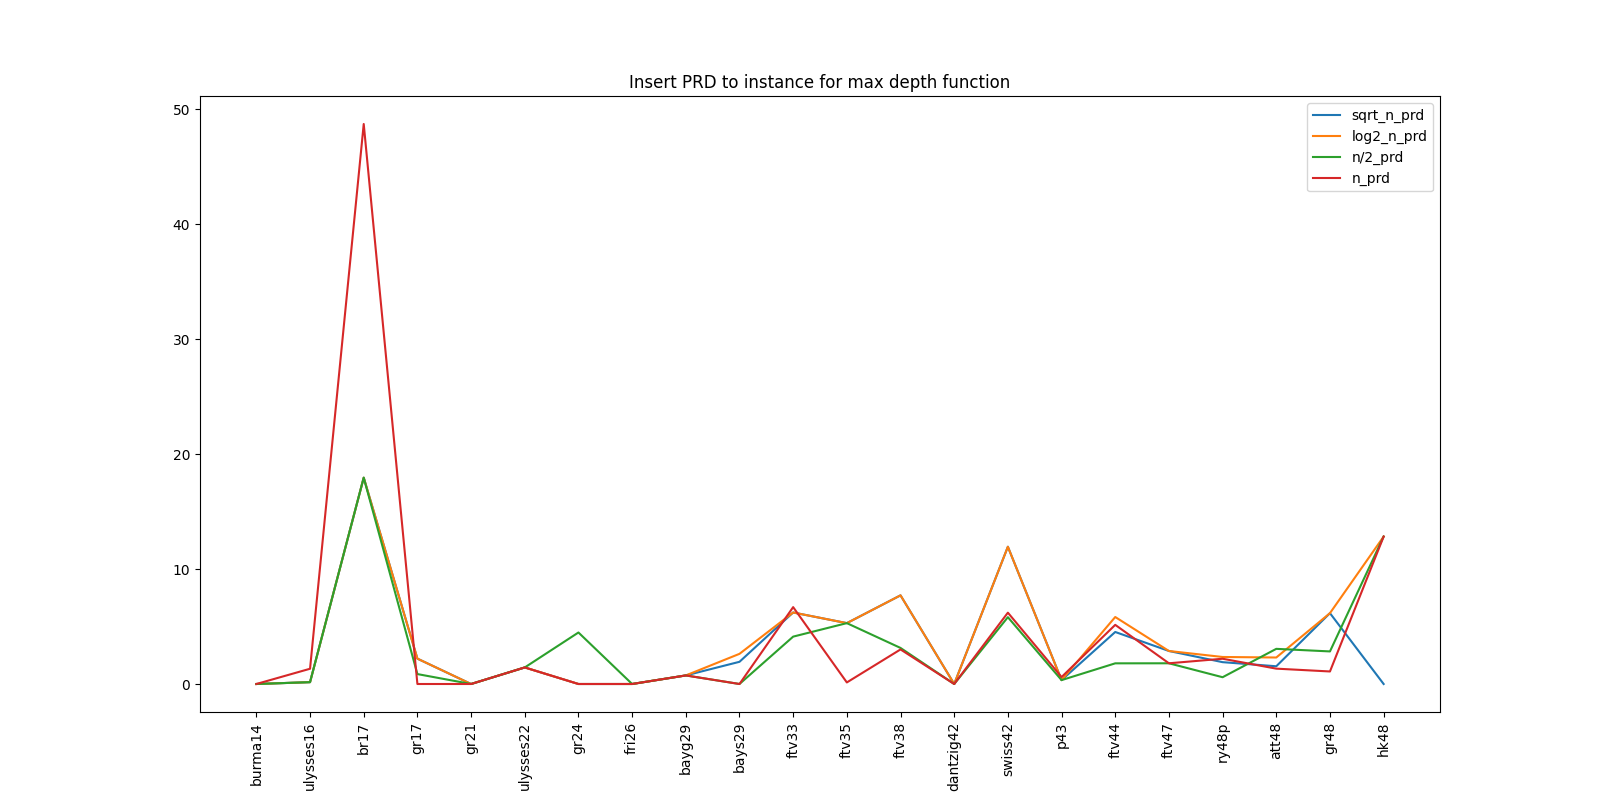
\includegraphics[scale=0.2]{depth_ins_prd.png}
      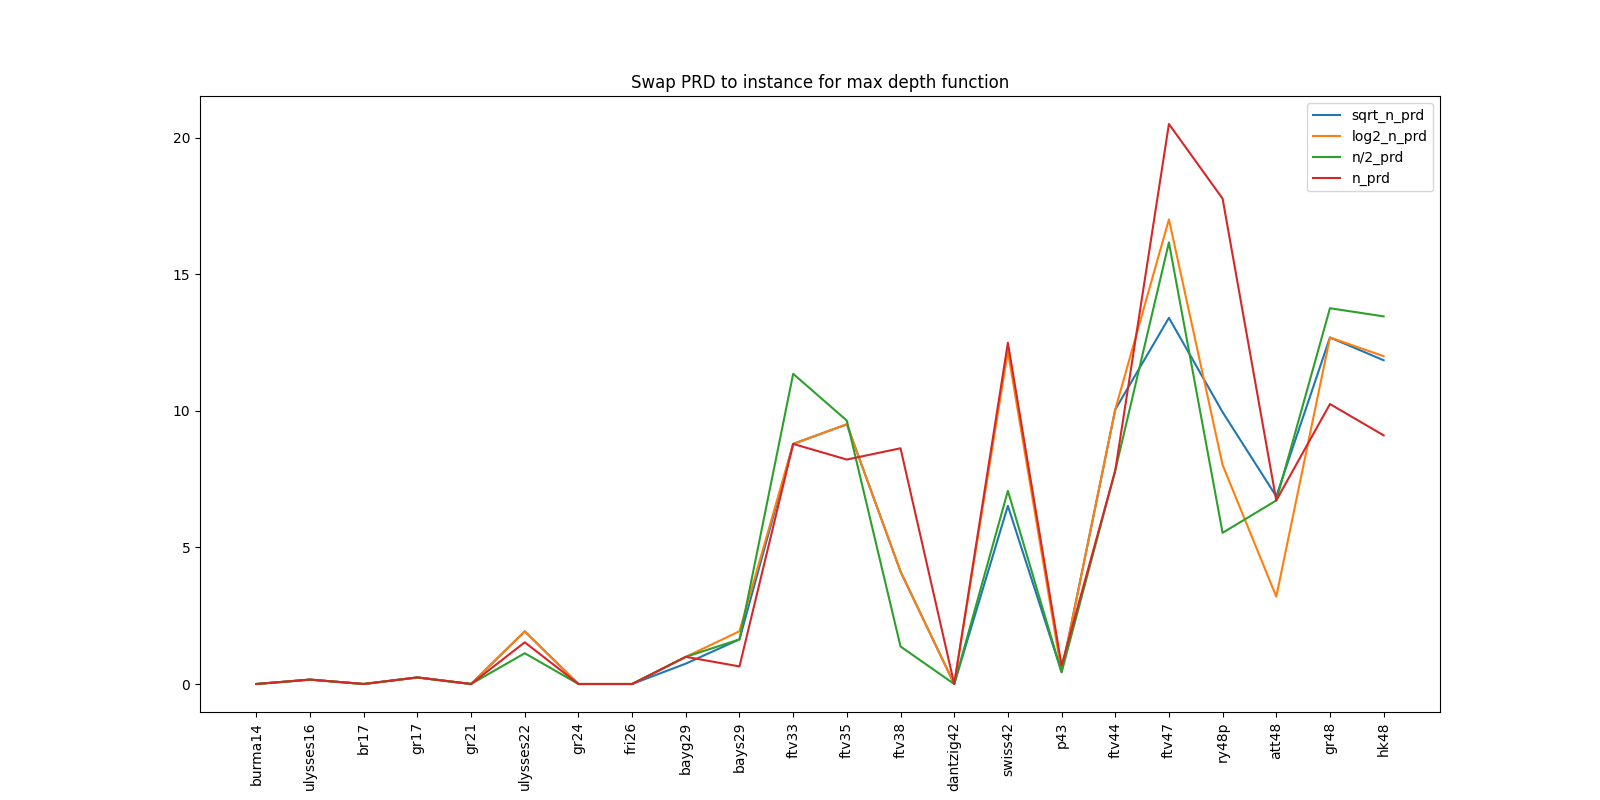
\includegraphics[scale=0.2]{depth_swp_prd.png}
    \end{center}
  \end{multicols}

W przypadku instancji losowych dla metody Invert najlepiej sprawdzały się funkcje
pierwiastka i logarytmu. Natomiast metody Swap oraz Insert faworyzowały większe wartości
funkcji i dawały najlepsze wyniki w okolicach wartości $n/2$.\\

Instancje TSPLib dla medtody Invert zachowywały się podobnie. Natomiast metoda Swap oraz
Insert często przyjmowały dobre wartości dla funcki $n/2$ jednak istniała duża ilość przypadków
gdzie inne funkcje radziły sobie lepiej. Możliwe, że jest to kwestia korelacji z innymi parametrami
wywołania które były opytmalizowane głównie pod metodę Invert.

\section{Wpłw maksymalnej liczby iteracji bez poprawy na PRD}

Na wykresach przedstawiono zależność prd od wielkości lub typu instancji dla różnych maksymalnych liczb iteracji bez poprawy.

\begin{multicols}{2}
    \begin{center}
      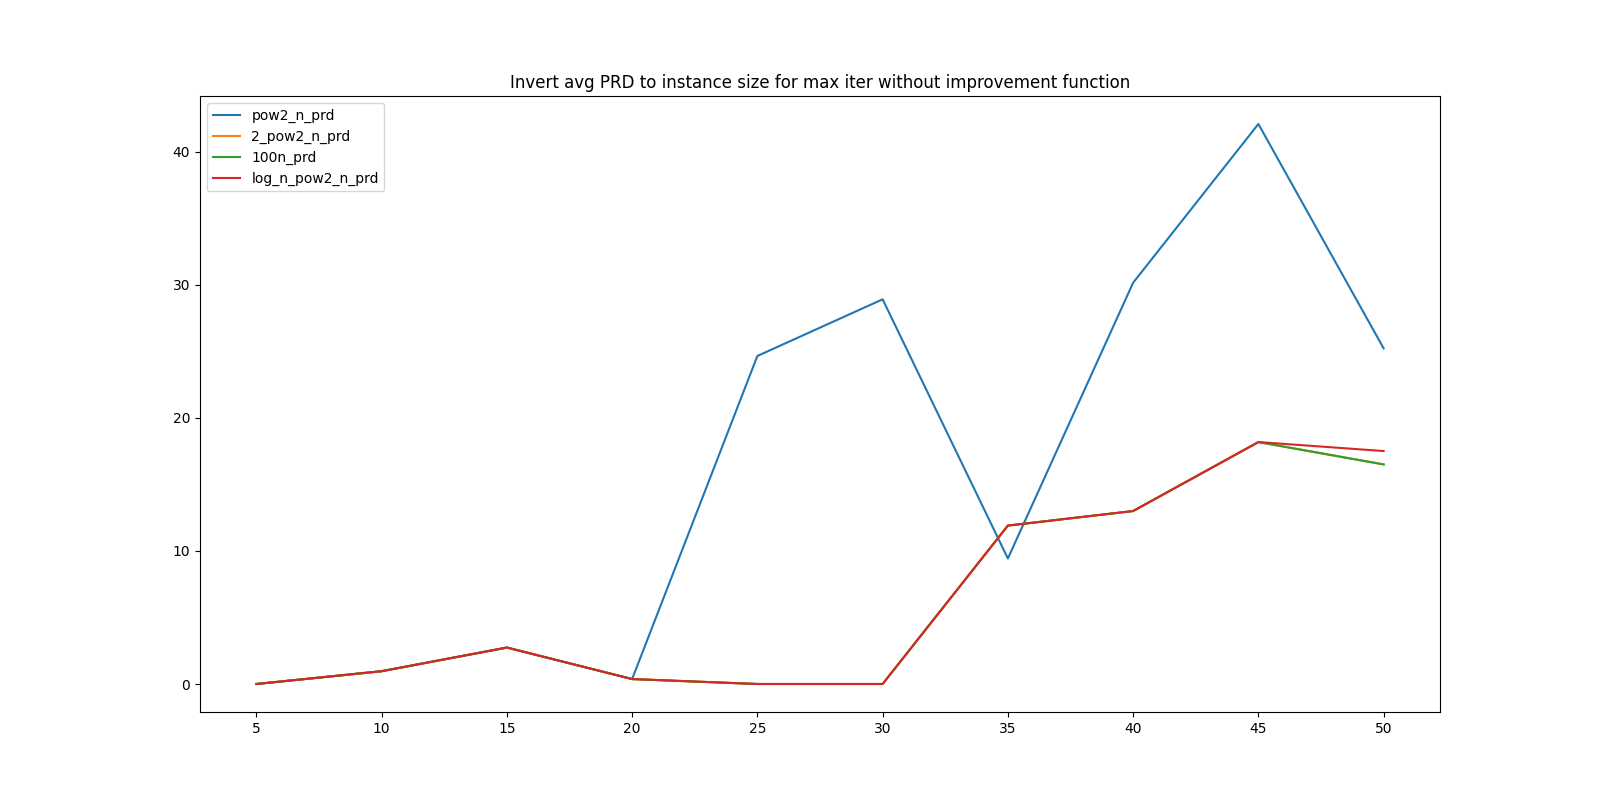
\includegraphics[scale=0.2]{rand_impiter_inv_prd.png}
      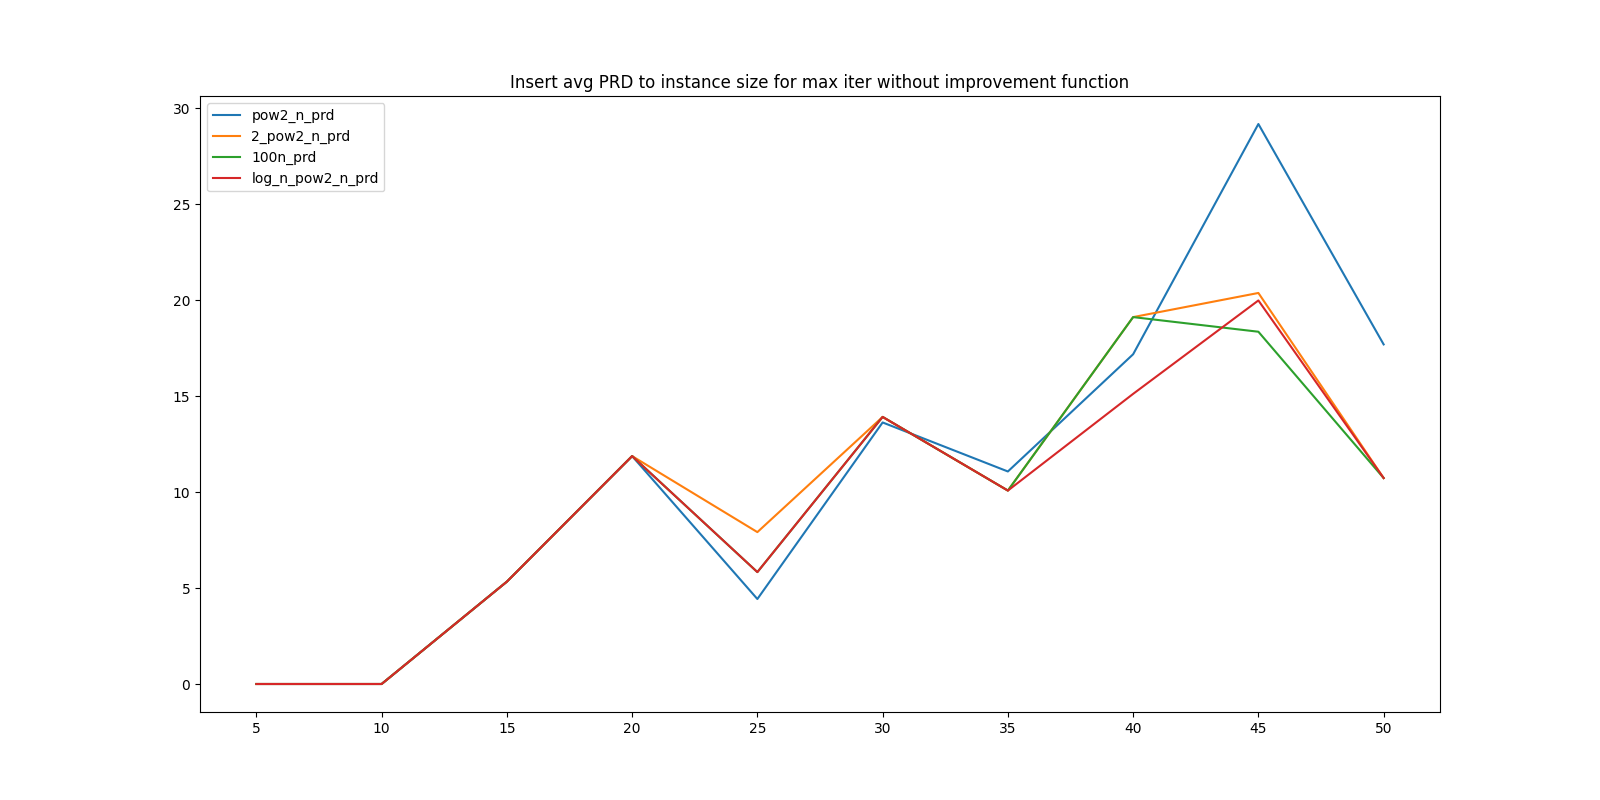
\includegraphics[scale=0.2]{rand_impiter_ins_prd.png}
      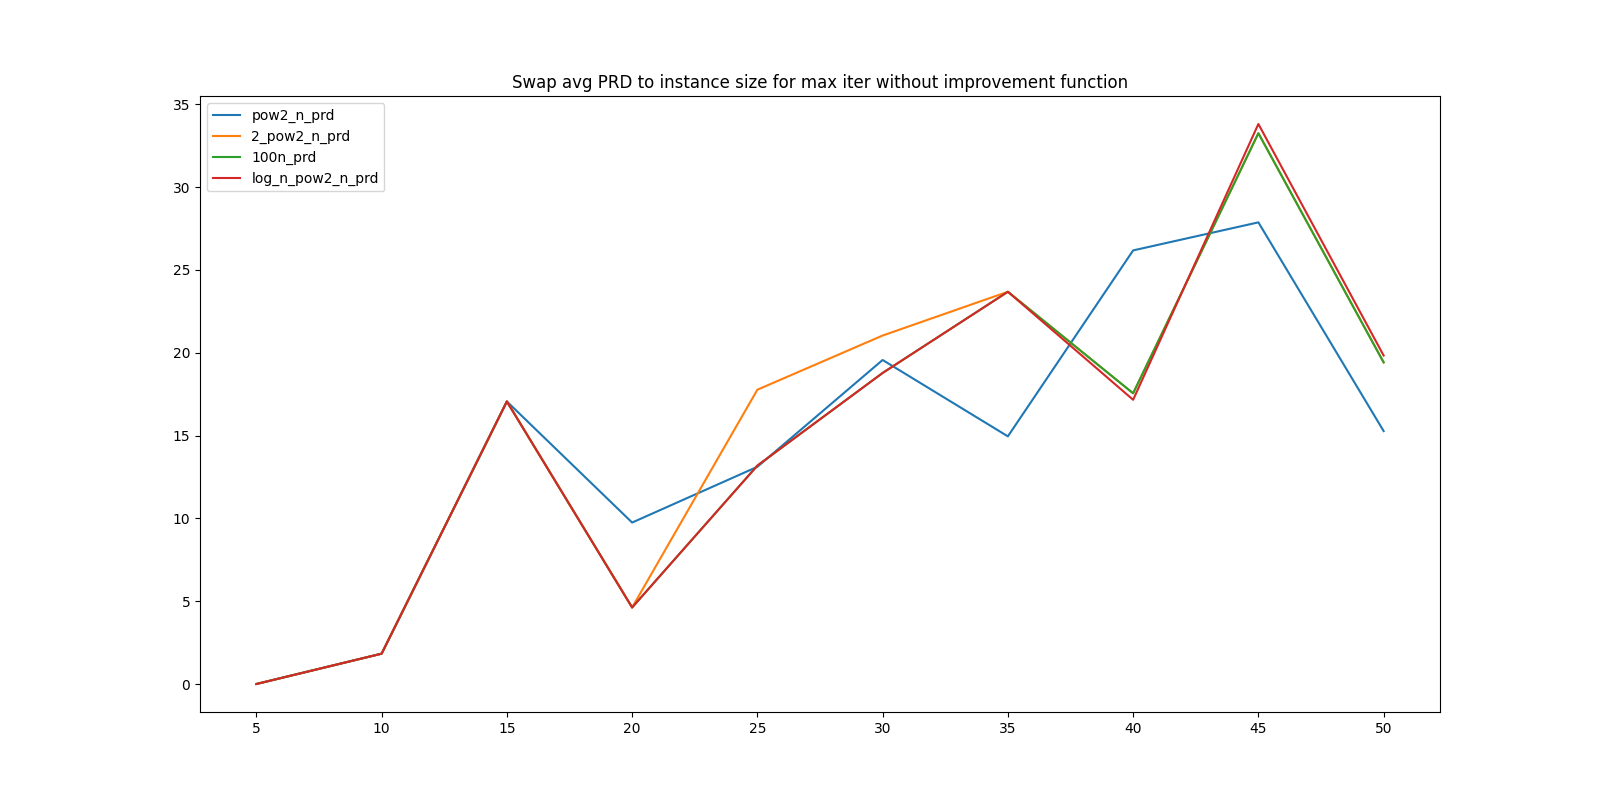
\includegraphics[scale=0.2]{rand_impiter_swp_prd.png}
      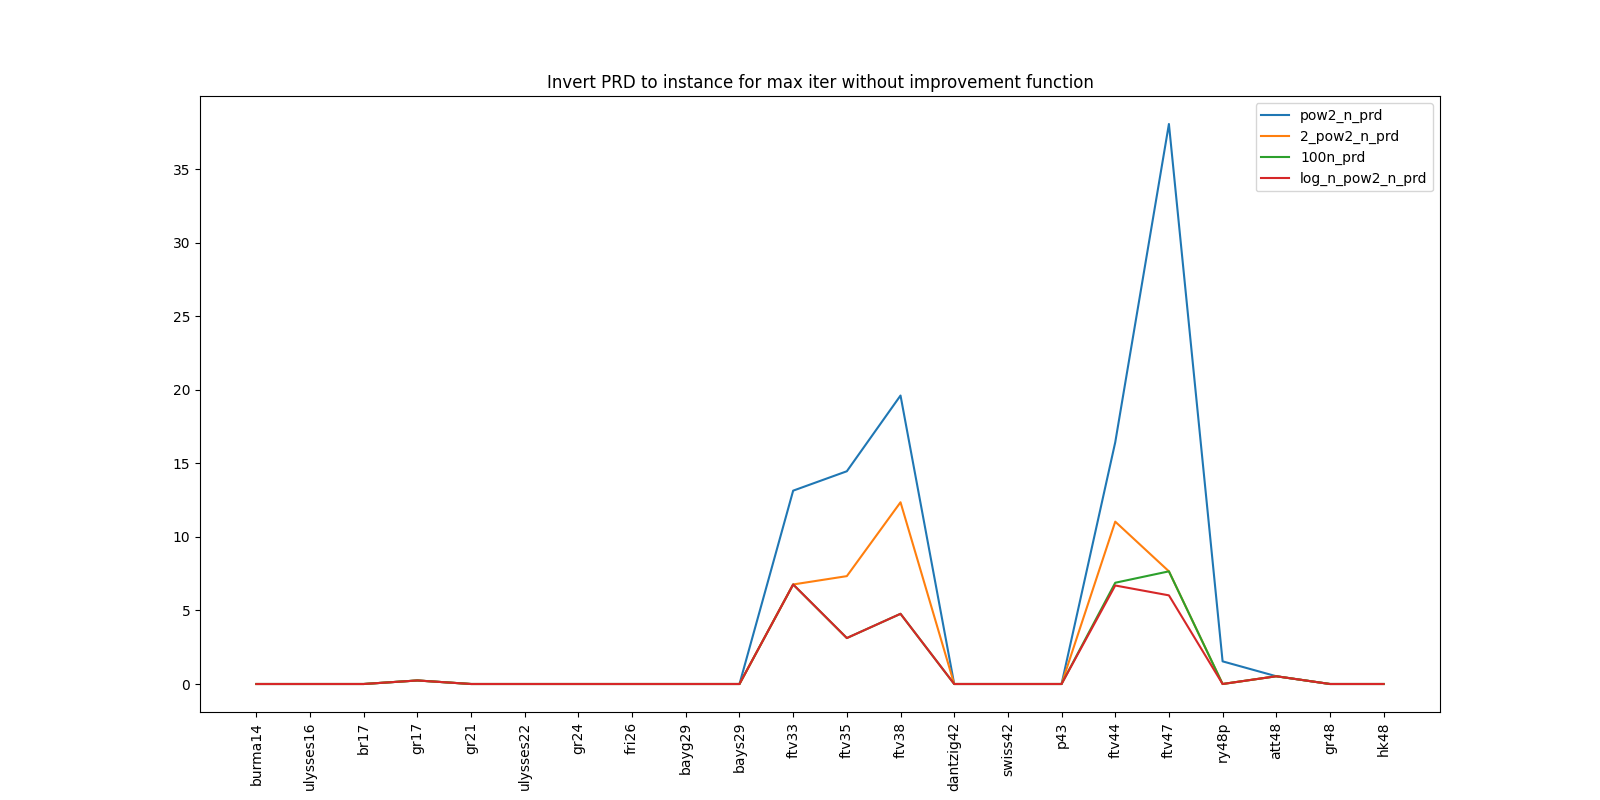
\includegraphics[scale=0.2]{impiter_inv_prd.png}
      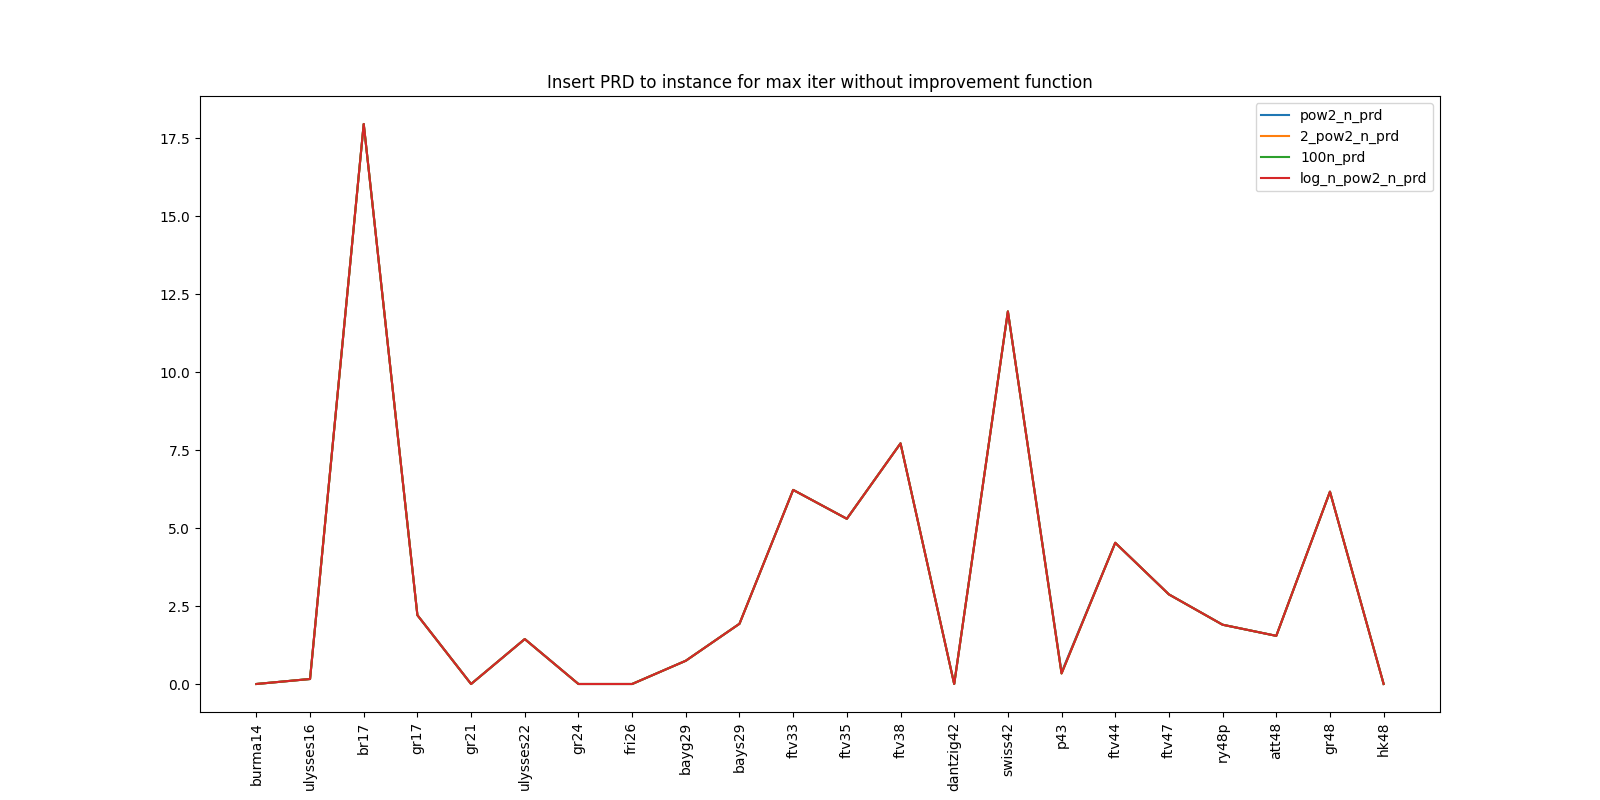
\includegraphics[scale=0.2]{impiter_ins_prd.png}
      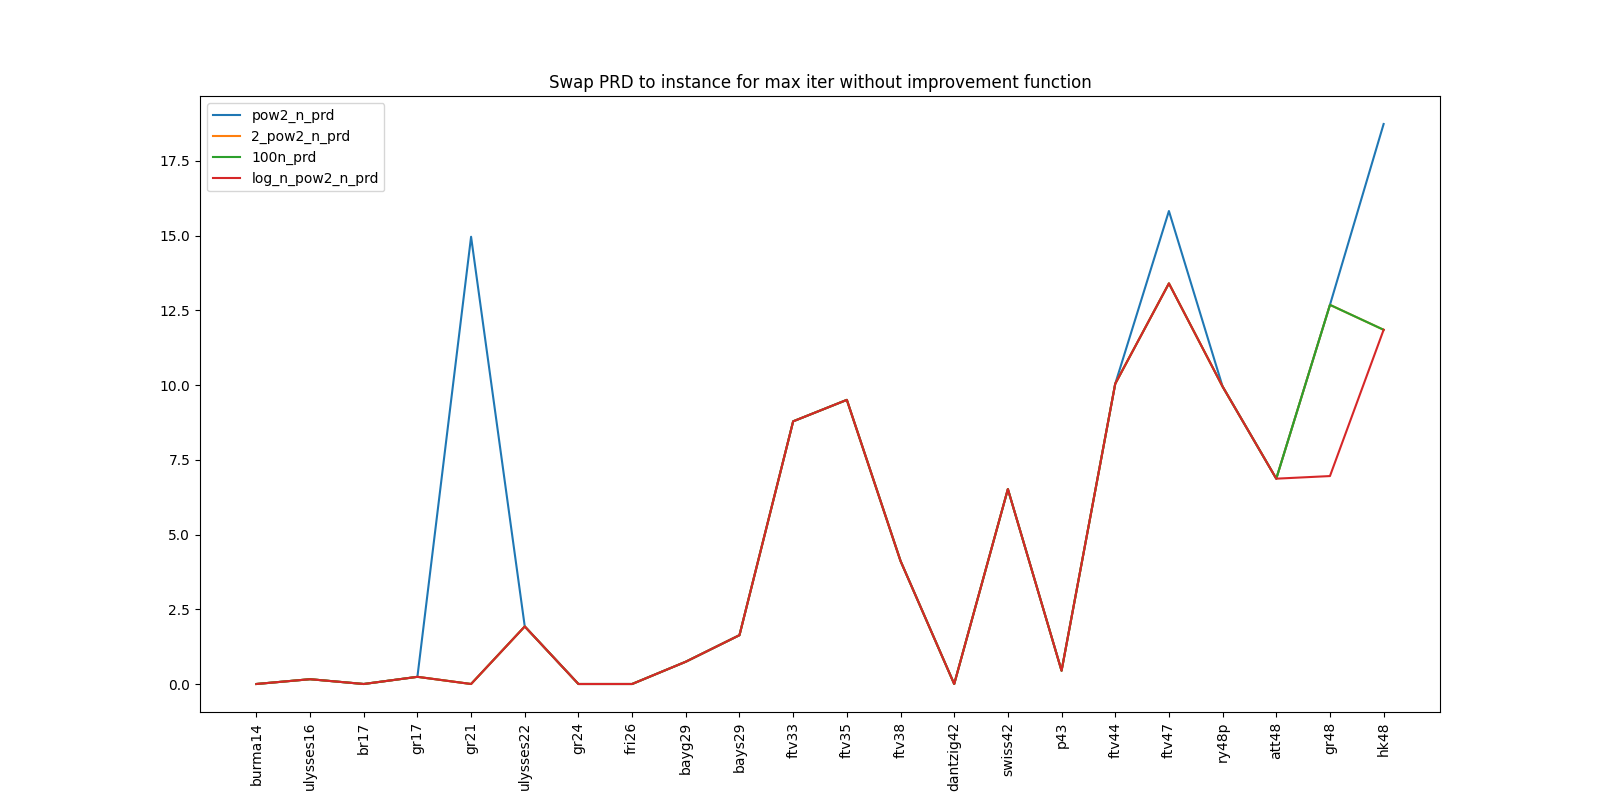
\includegraphics[scale=0.2]{impiter_swp_prd.png}
  \end{center}
\end{multicols}
Metoda Invert faworyzowała największą z funkcji czyli $\log(n) * n^2$. Metoda Insert
zahowywała się podobnie. Natomiast metoda Swap nie wykazała aby konkretna funkcja dawała
lepsze wartości co jak w poprzednich przypadkach może być związane z doborem pozostałych
parametrów.\\

W pzrypadku instancji TSPLib dobrze widać, że funkcja $\log(n) * n^2$ sprawuje się najlepiej
dla metody Invert. Szczególnie polepsza ona wyniki w przypadku instancji asymetrycznych. Pozostałe
metody podobnie jak powyżej wymagają głebszych badań pod kątem specyfiki problemu i doboru parametrów.
\\~\\
Ciekawym spostrzeżeniem okazał się fakt (niestety nie zawarty na wykresach) iż dla niektórych
instancji osiągana została maksymalna liczba iteracji. Po uruchomieniu tych instncji z większym limitem iteracji
można było zaobserwować znaczące poprawy wyników. Badanie to jednak nie zostało ukończone głównie ze
względu na ilości czasu potrzebne na liczenie dużych instancji z taką ilością iteracji.

\end{document}